% !TEX root = DesignDocument.tex


\chapter{Prototypes}

This chapter is for recording each prototype developed.  It is a historical record of what you accomplished in 464/465.   This should be organized according to Sprints.  It should have the basic description of the sprint deliverable and what was accomplished.  Screen shots, photos, captures from video, etc should be used.  

\section{Sprint 1 Prototype}
This sprint was focused on learning Android and iOS development tools, as well as designing the UX and the database schema.
\subsection{Deliverable}
	\begin{itemize}
		\item UX for Android
		\item UX for iOS
	\end{itemize}
\subsection{Backlog}
	\begin{itemize}
		\item UX design (MVC)
		\begin{itemize}
			\item Create group
			\item Leave group
			\item Group messaging
			\item Start page
		\end{itemize}
		\item Database
		\begin{itemize}
			\item Design database schema
			\item Implement database on Parse
		\end{itemize}
	\end{itemize}
\subsection{Success/Fail}
\begin{itemize}
	\item Designs for Create Group page
	\item Design for Leave Group page
	\item Design for Group Messaging page
	\item Design for Start Page
	\item Design for Database Schema
	\item Database implementation
	\item Git Repository Initialization
\end{itemize}

\section{Sprint 2 Prototype}

	\begin{figure}[tbh]
	\begin{center}
	\fbox{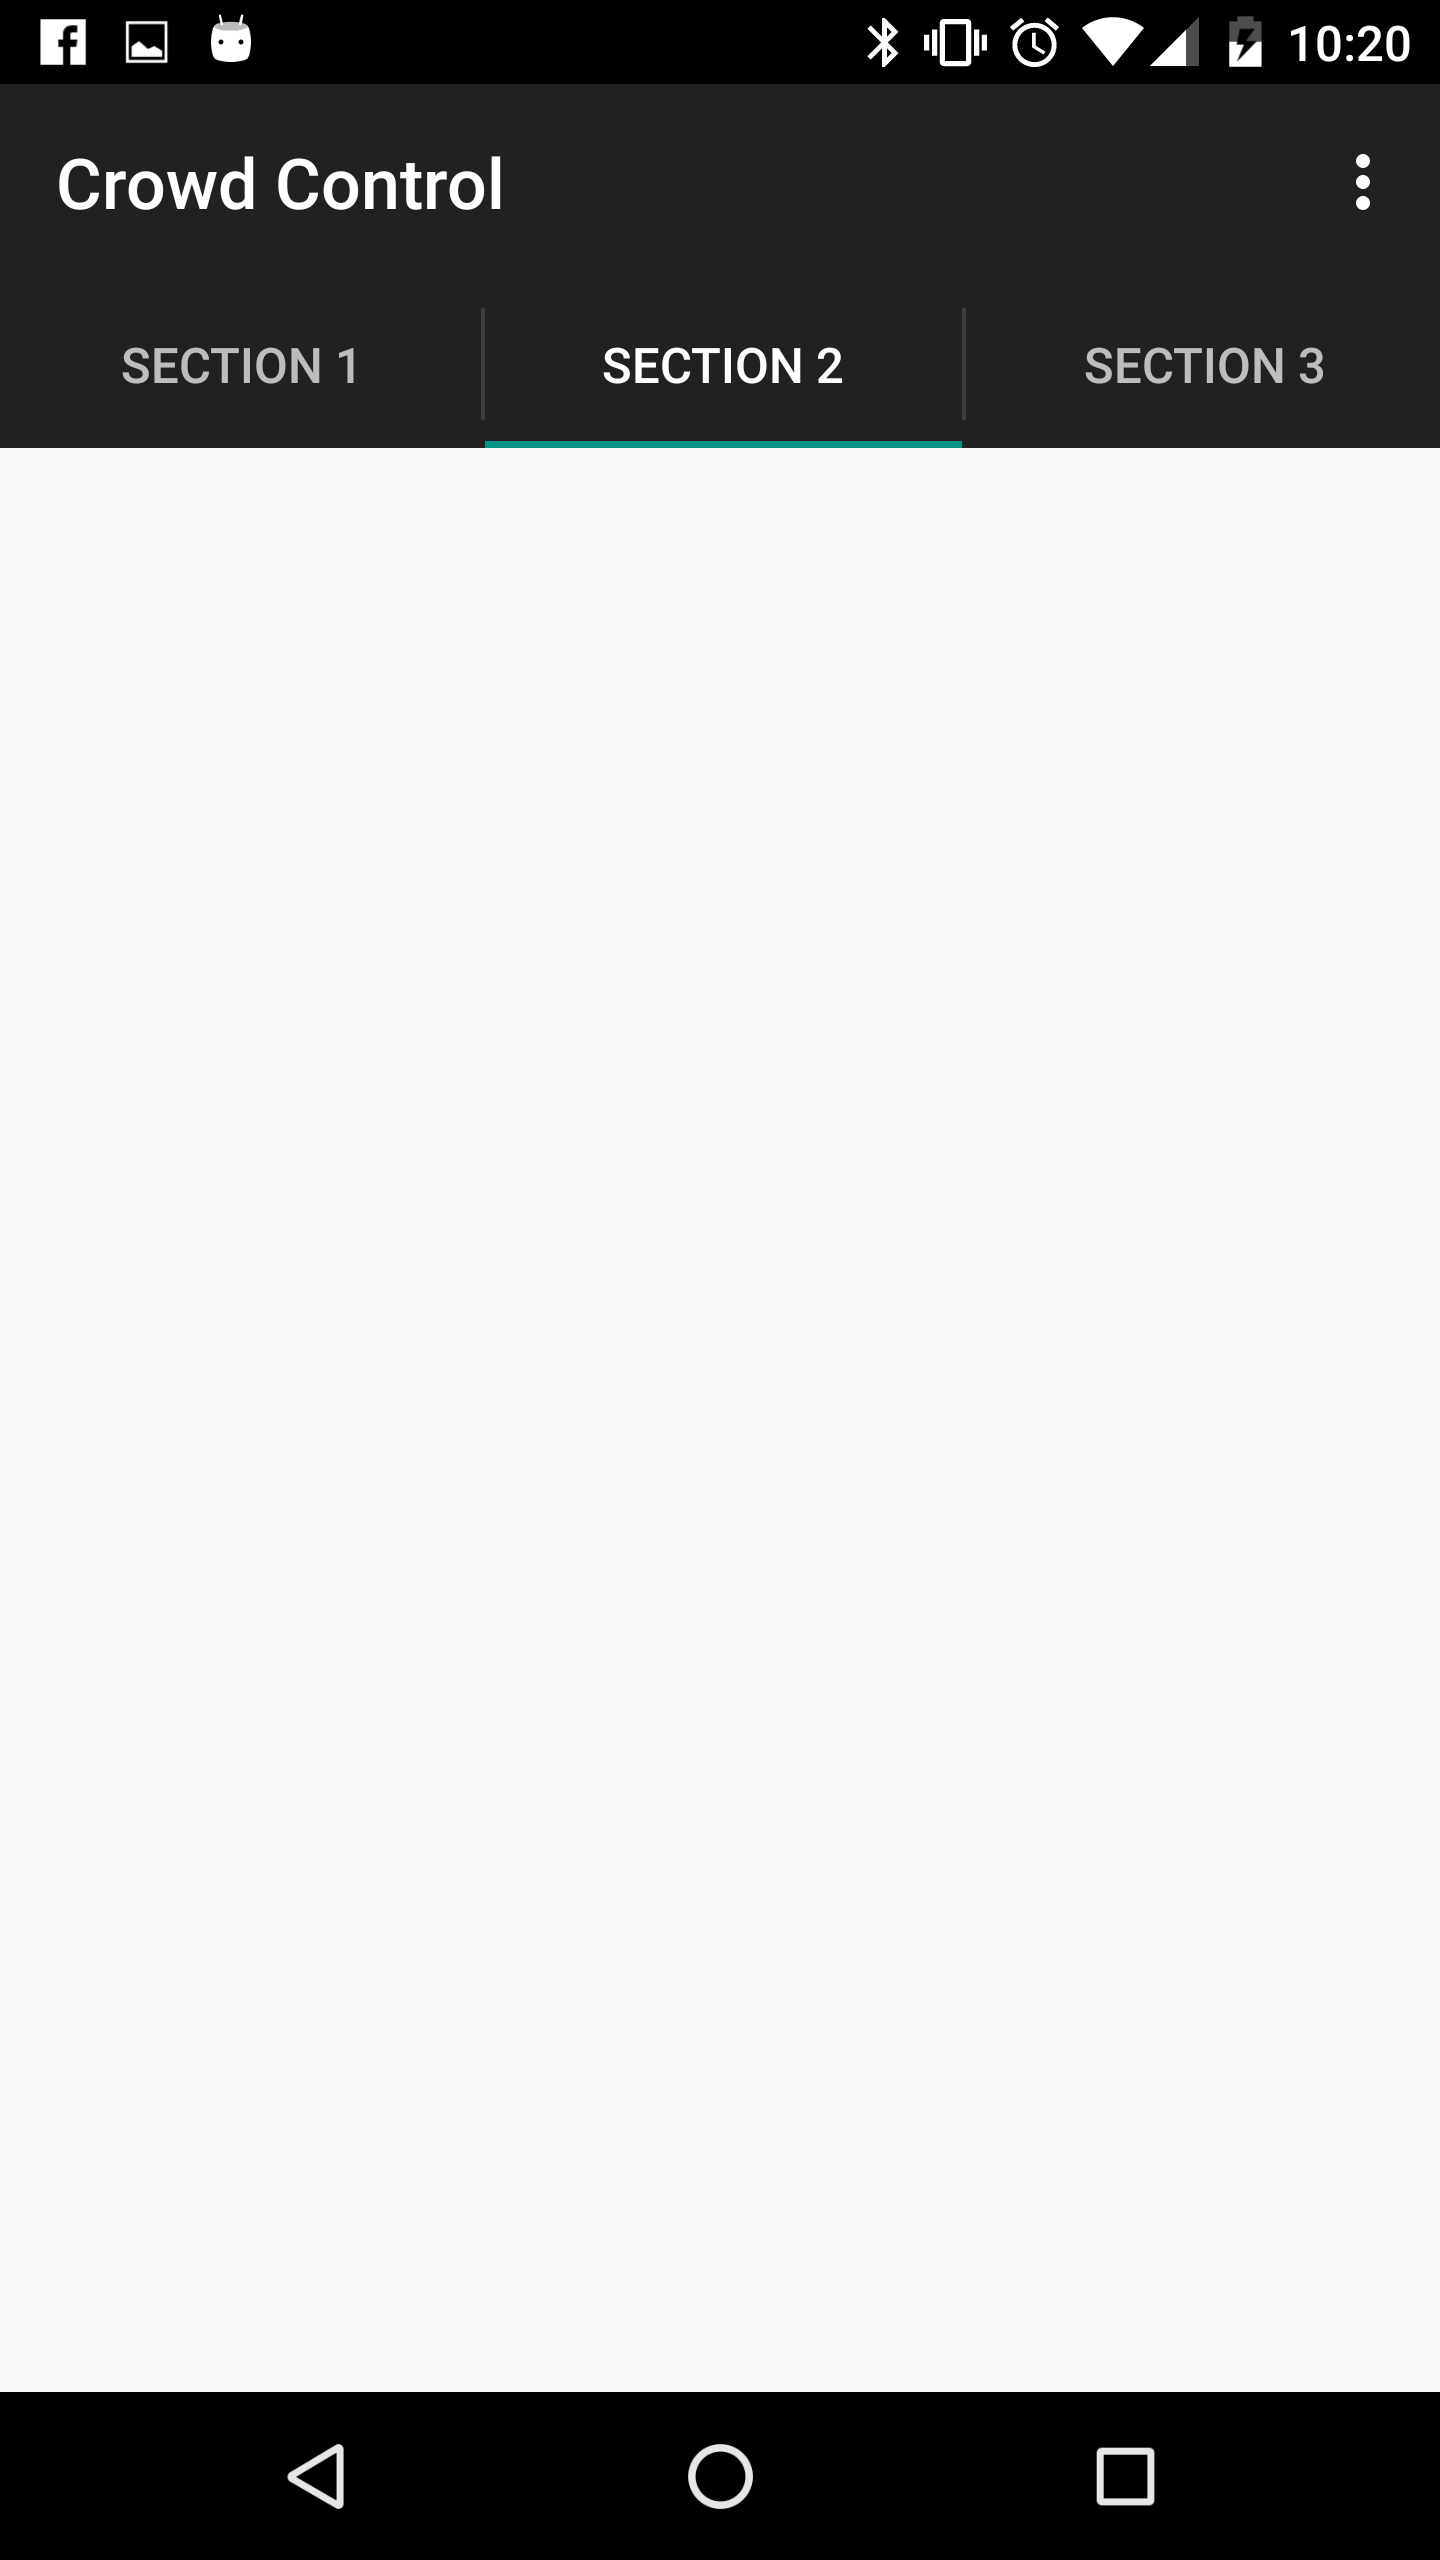
\includegraphics[scale=.1]{Additional/Prototypes/Sprint2/tabs.PNG}}
	\end{center}
	\caption{Sprint 2 Prototypes. \label{CommFlow}}
	\end{figure}

\subsection{Deliverable}
\begin{itemize}
	\item Android
	\begin{itemize}
		\item UX
		\begin{itemize}
			\item Designed map screen
			\item Designed group info screen
			\item Designed start page
			\item Designed group messaging
			\item Created initial tabs holder
		\end{itemize}
		\item Model
		\begin{itemize}
			\item Created skeleton user model
			\item Created skeleton group model
			\item Created skeleton abstractions for models
		\end{itemize}
	\end{itemize}
	\item iOS
	\begin{itemize}
		\item UX
		\begin{itemize}
			\item Created map display
			\item Added homing button to map display
			\item Created simple group display
		\end{itemize}
		\item Model
		\begin{itemize}
			\item Created skeleton user model
			\item Created skeleton profile model
			\item Created skeleton group model
			\item Created skeleton abstractions for models
		\end{itemize}
	\end{itemize}
	\item Parse
	\begin{itemize}
		\item Created User table
		\item Created CCUser table
		\item Created Group table
	\end{itemize}
	\item Work was also done on the Business Plan
\end{itemize}
\subsection{Backlog}
\begin{itemize}
	\item Code UX
	\begin{itemize}
		\item Implement mapping features
		\item Create messaging UI
	\end{itemize}
	\item Model
	\begin{itemize}
		\item Create user Model
		\item Create communication Layer
		\item Link back-end and front end
	\end{itemize}
	\item Create parse tables
	\item Business Plan
\end{itemize}
\subsection{Success/Fail}
\begin{itemize}
	\item We had a hard time finding a version of Public/Private key encryption that fit our project.
	\item Differences between iOS and android coding standards made it hard to create a similar look and feel.
	\item iOS is simply easier to make these initial pieces in, and has jumped far ahead android.
	\item iOS map features are proving very difficult to test.
\end{itemize}

\section{Sprint 3 Prototype}

	\begin{figure}[tbh]
	\begin{center}
	\fbox{\includegraphics[scale=.1]{Additional/Prototypes/Sprint3/createAccount.PNG}}
	\fbox{\includegraphics[scale=.1]{Additional/Prototypes/Sprint3/email.PNG}}
	\end{center}
	\caption{Sprint 3 Prototypes. \label{CommFlow}}
	\end{figure}

\subsection{Deliverable}
\begin{itemize}
	\item iOS
	\begin{itemize}
		\item Created a log-in system
		\begin{itemize}
			\item Added ability to create a user
			\item Added Facebook integration for user creation
		\end{itemize}
		\item Added ability for users to join an existing group
	\end{itemize}
	\item Android
	\begin{itemize}
		\item Added ability to create a user with an email address
		\item Added group functionality
		\begin{itemize}
			\item Added a way for groups to be created
			\item Added a group join feature
		\end{itemize}		
	\end{itemize}
	\item Server
	\begin{itemize}
		\item Fixed connection issues between parse and app
		\item User table and profile(CCUser) are connected by apps in parse
	\end{itemize}
	\item Prepped business plan for SDSM\&T Business Plan Competition
\end{itemize}
\subsection{Backlog}
\begin{itemize}
	\item Install a messaging API
	\item Allow users to join a group
	\item Cloud Code
	\begin{itemize}
		\item Create safe group operations
		\item Link user information
	\end{itemize}
	\item Business Plan
	\begin{itemize}
		\item Submit to SDSM\&T Business Plan Competition
		\item Prep for South Dakota Giant Vision
	\end{itemize}
\end{itemize}
\subsection{Success/Fail}
\begin{itemize}
	\item Failures
	\begin{itemize}
		\item Not all of the group functionality is working properly
		\item We were unable to get to messaging this sprint
	\end{itemize}
	\item Changes
	\begin{itemize}
		\item Rewrote the database schema
		\item Modified GUI appearance
	\end{itemize}
	\item Successes
	\begin{itemize}
		\item iOS was successful in connecting to Facebook
		\item Android managed to start creating groups
		\item Our business plan was accepted by SDSM\&T Business Plan Competition
	\end{itemize}
\end{itemize}

\section{Winter Sprint Prototype}

	\begin{figure}[tbh]
	\begin{center}
	\fbox{\includegraphics[scale=.1]{Additional/Prototypes/SprintW/createAccount.PNG}}
	\fbox{\includegraphics[scale=.1]{Additional/Prototypes/SprintW/email.PNG}}
	\fbox{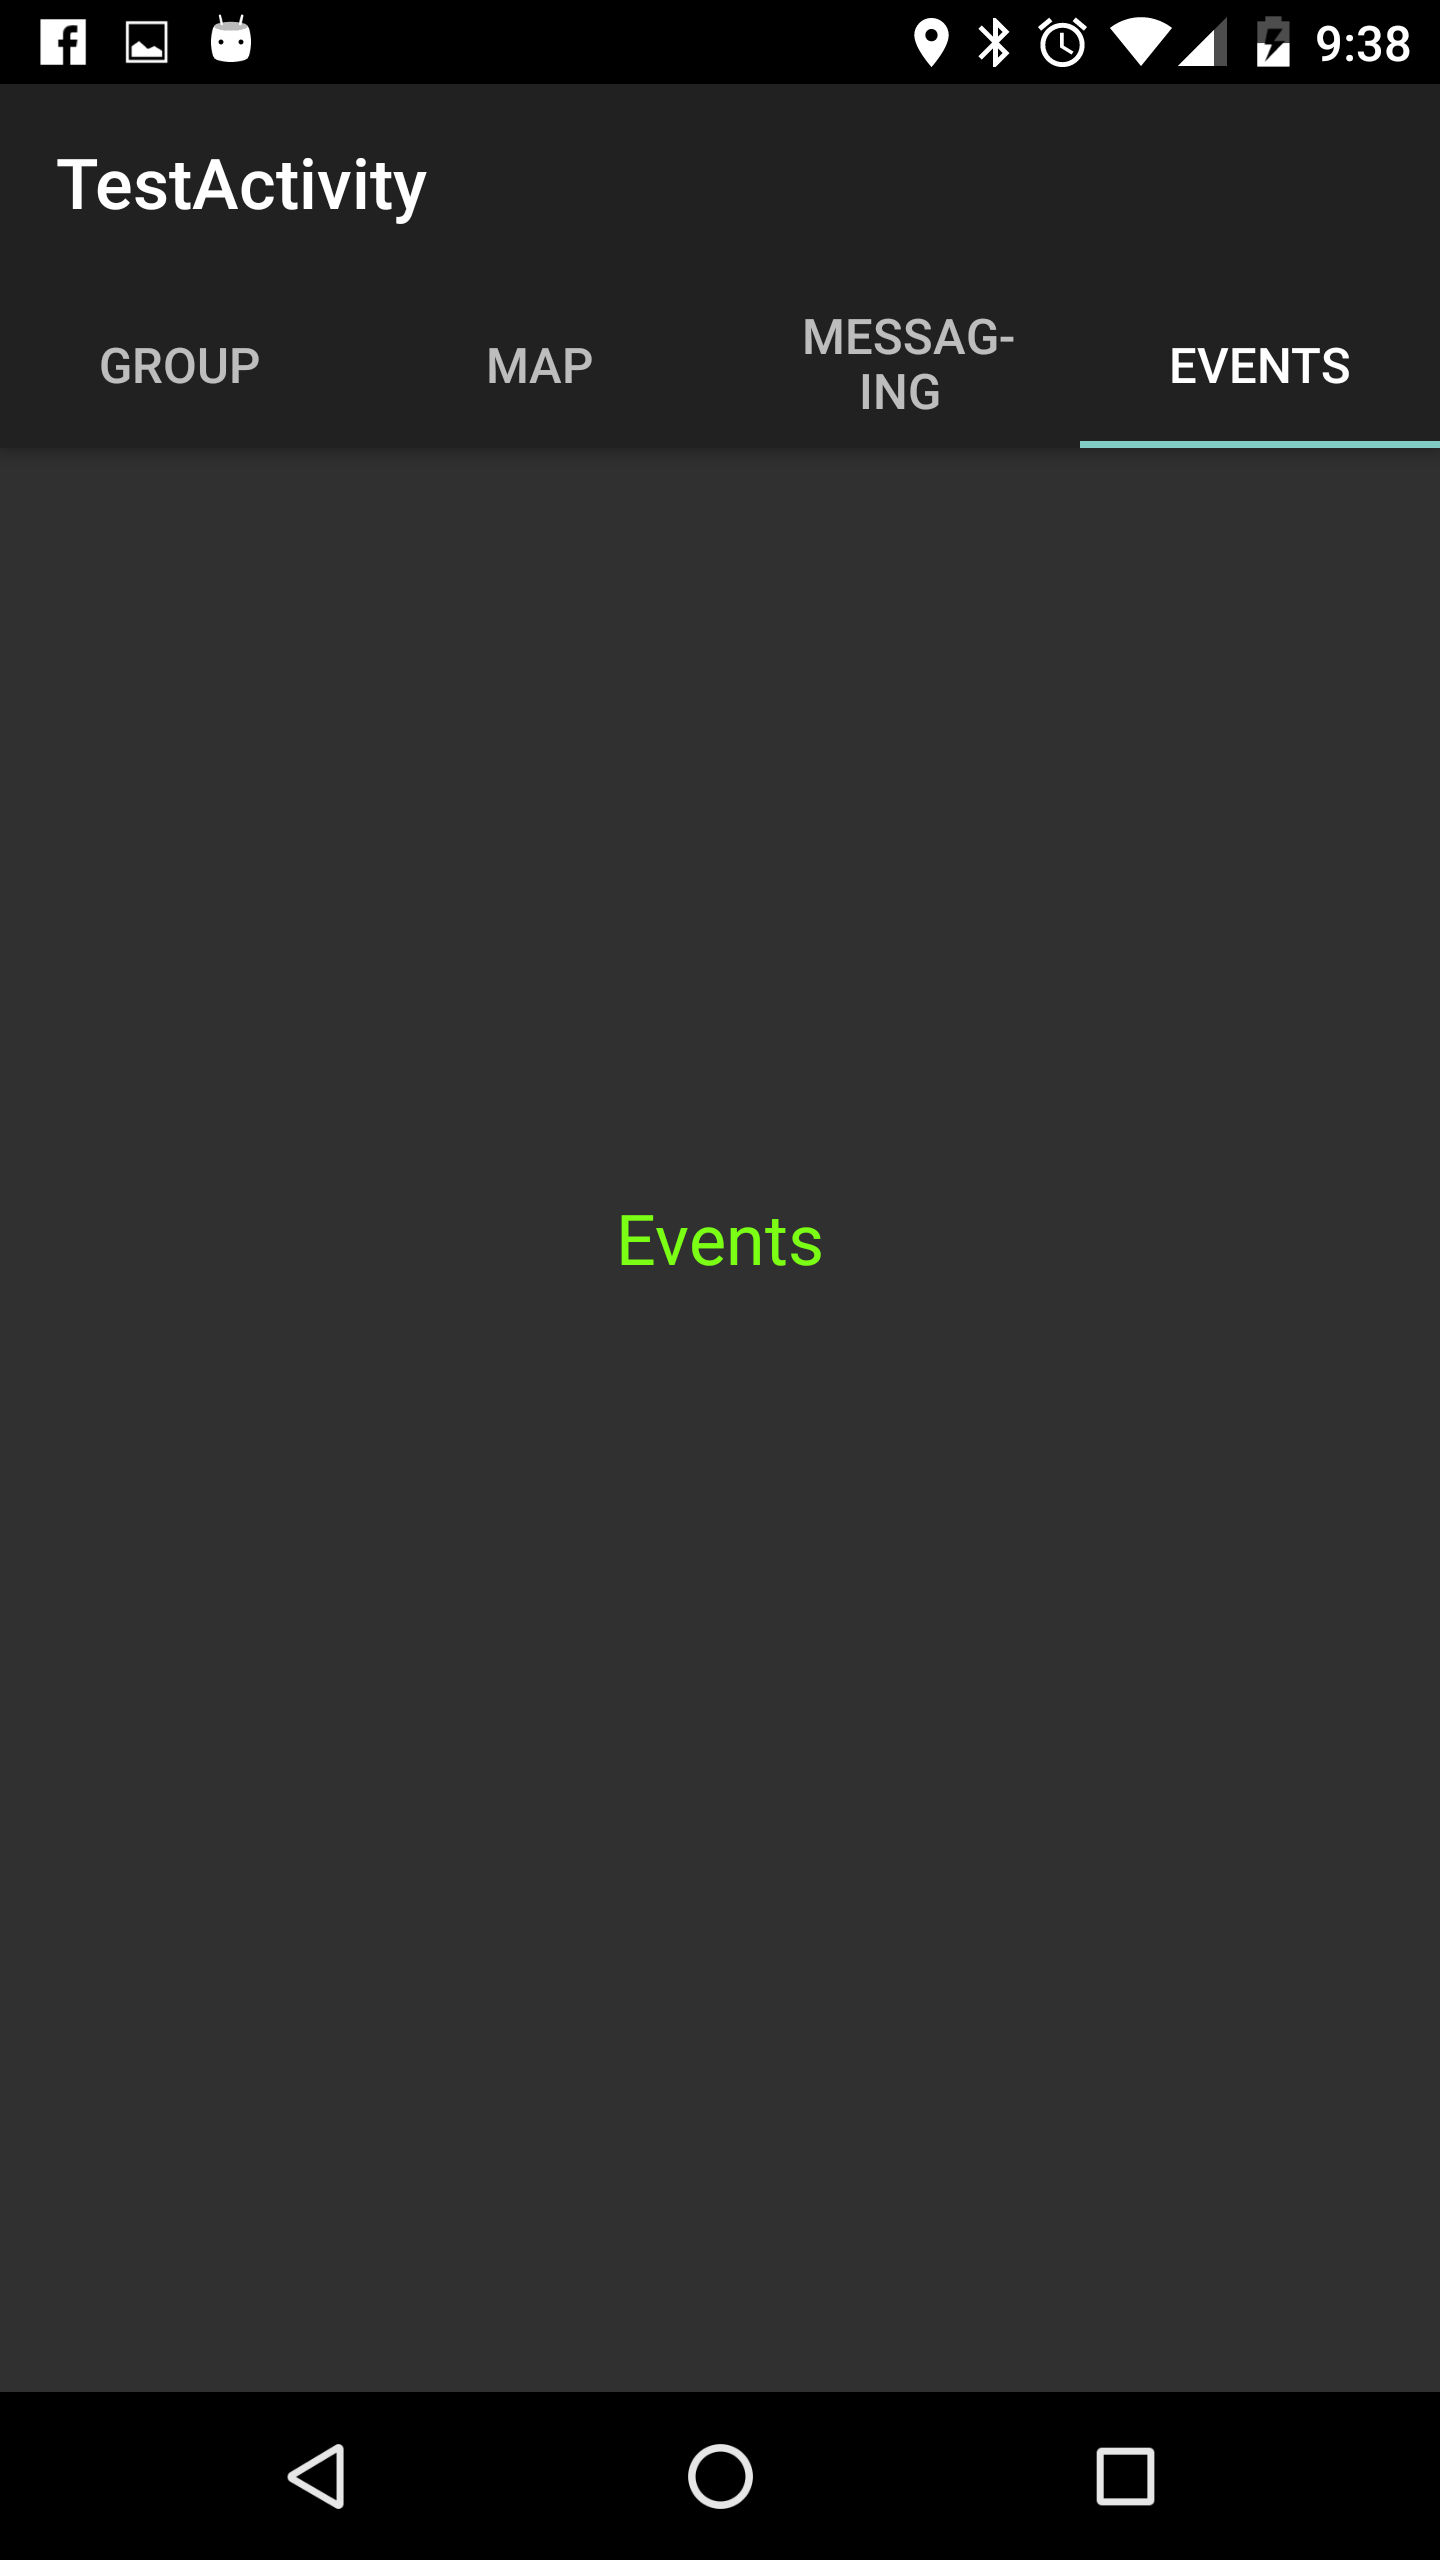
\includegraphics[scale=.1]{Additional/Prototypes/SprintW/events.PNG}}
	\fbox{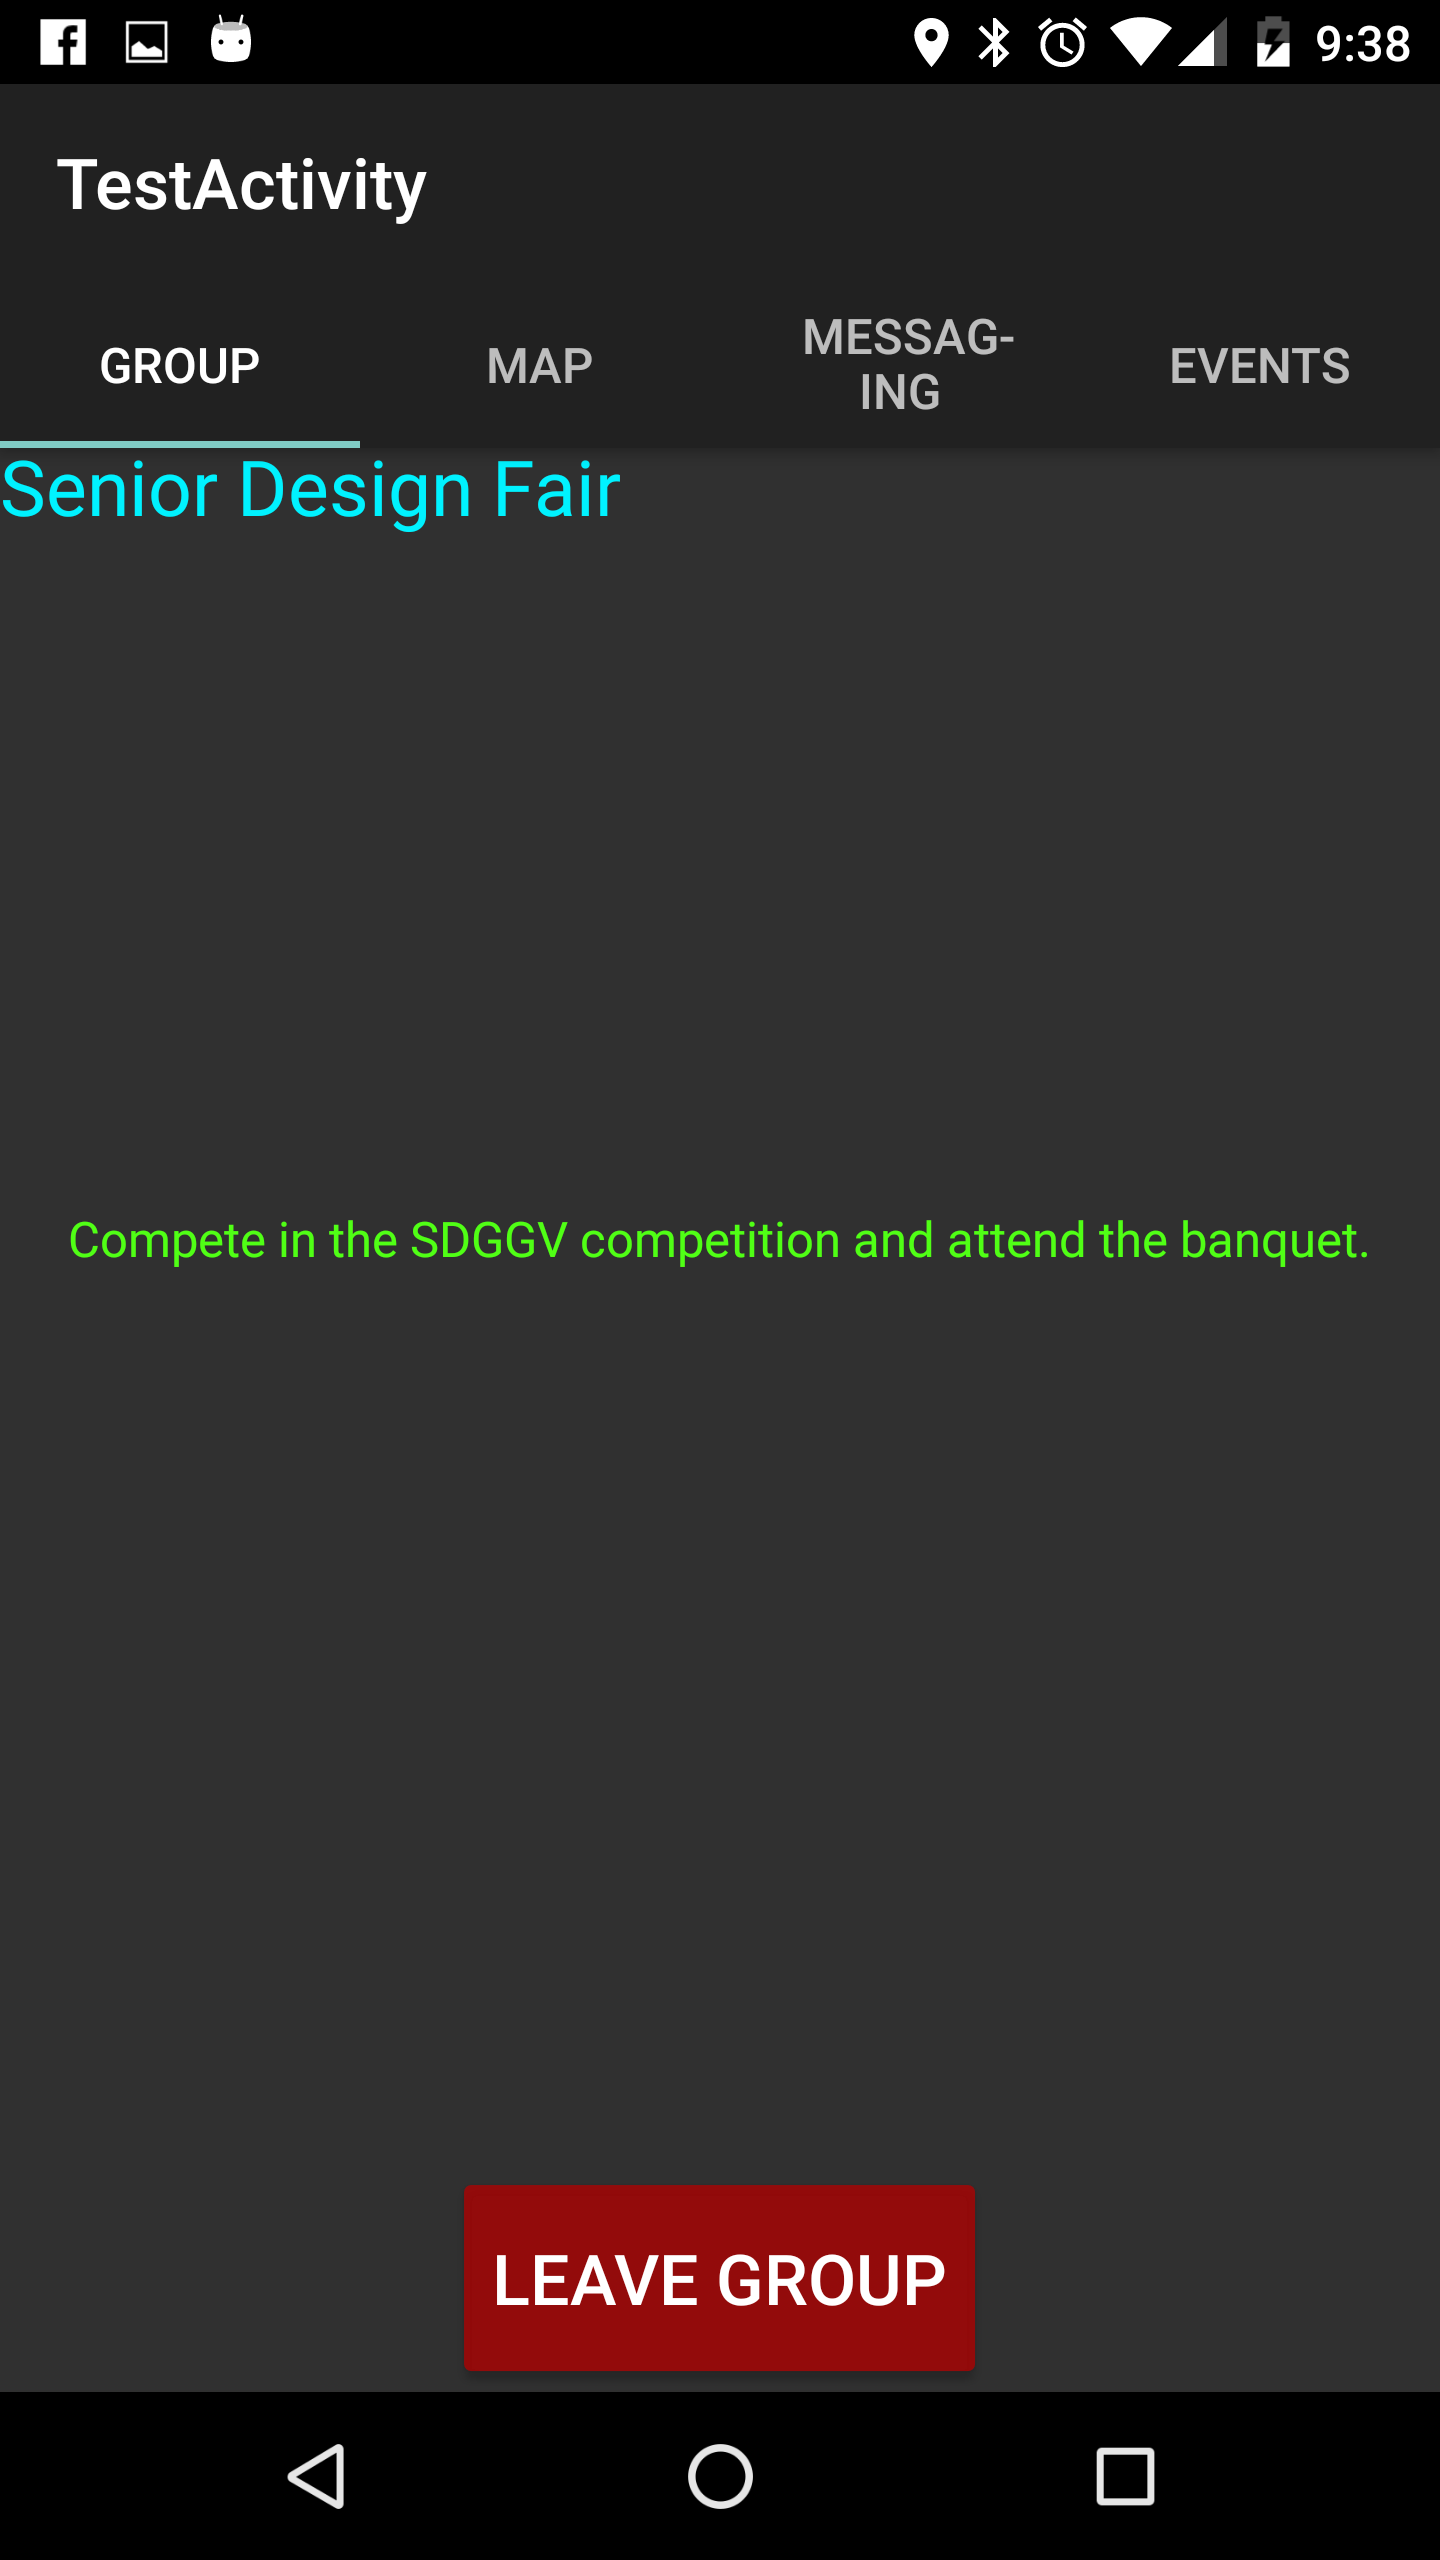
\includegraphics[scale=.1]{Additional/Prototypes/SprintW/info.PNG}}
	\fbox{\includegraphics[scale=.1]{Additional/Prototypes/SprintW/join.PNG}}
	\fbox{\includegraphics[scale=.1]{Additional/Prototypes/SprintW/messaging.PNG}}
	\end{center}
	\caption{Winter Sprint Prototypes. \label{CommFlow}}
	\end{figure}

\subsection{Deliverable}
\begin{itemize}
	\item iOS
	\begin{itemize}
		\item Log-in/Log-out
		\begin{itemize}
			\item Improved Log-in/sign-up screens
			\item Added Log-out feature
		\end{itemize}
		\item Settings
		\begin{itemize}
			\item Implemented settings screen
			\item Nested log-out functionality into settings screen
		\end{itemize}
		\item Groups
		\begin{itemize}
			\item Implemented leaving/Joining a group
			\item Improved basic group operations
			\item Detects if users are in a group
		\end{itemize}
	\end{itemize}
	\item Android
	\begin{itemize}
		\item Log-in
		\begin{itemize}
			\item Automatic log-in on start-up (from data-store)
			\item Log-in to existing account via email address
		\end{itemize}
		\item Settings
		\begin{itemize}
			\item Page layout created and linked from GroupJoin page
			\item Log-out functionality implemented
		\end{itemize}
		\item Groups
		\begin{itemize}
			\item Leave button implemented
			\item Tested adding/removing users from groups
		\end{itemize}
	\end{itemize}
	\item Misc/Transitional
	\begin{itemize}
		\item Further documented Android code to prepare for team merge
		\item Android code review with iOS team, to prepare for team merge
	\end{itemize}
\end{itemize}
\subsection{Backlog}
\begin{itemize}
	\item Android
	\begin{itemize}
		\item Messaging (Sinch API)
		\item GPS Location (back-end models)
		\item Persistent groups through local data-store
	\end{itemize}
	\item iOS
	\begin{itemize}
		\item Messaging (Sinch API)
	\end{itemize}
\end{itemize}
\subsection{Success/Fail}
\begin{itemize}
	\item 
	\begin{itemize}
		\item Messaging wasn't touched
		\item Android is still missing GPS location work
		\item User does not automatically connect to a group if they are in one
	\end{itemize}
	\item Successes
	\begin{itemize}
		\item Android
		\begin{itemize}
			\item Log-in through email
			\item Settings page (layout and implementation)
			\item Local Data-store (individual automatic log-in)
		\end{itemize}
		\item iOS
		\begin{itemize}
			\item Log-in/Log-out
			\item Settings page (layout and implementation)
			\item Group functionality written
		\end{itemize}
	\end{itemize}
\end{itemize}

\section{Sprint 4 Prototype}

	\begin{figure}[tbh]
	\begin{center}
	\fbox{\includegraphics[scale=.1]{Additional/Prototypes/Sprint4/join.PNG}}
	\fbox{\includegraphics[scale=.1]{Additional/Prototypes/Sprint4/messaging.PNG}}
	\end{center}
	\caption{Sprint 4 Prototypes. \label{CommFlow}}
	\end{figure}

\subsection{Deliverable}
\begin{itemize}
	\item Android
	\begin{itemize}
		\item Group Messaging
		\begin{itemize}
			\item Created a Layout
			\item Used Sinch code to create a service
			\item Implemented group messaging
			\item Group messaging is working with no known bugs
			\end{itemize}
		\item Location
		\begin{itemize}
			\item Page layout created and linked from GroupJoin page
			\item MapFragment has buttons for homing and syncing group locations
			\item Retrieving the user's location on instantiation of the MapFragment
			\item User and group locations implemented
		\end{itemize}
		\item Group update service
		\begin{itemize}
			\item Checks for updates in near real-time
			\item Updates group settings when changed
			\item Updates group members if someone leaves or joins
		\end{itemize}
	\end{itemize}
	\item Server (cloud code)
	\begin{itemize}
		\item Functional Group update indicator
		\item Returning group update information
		\item Join group function (created but not functioning)
		\item Leave group function (created but not functioning)
		\item Check for Existing Email
	\end{itemize}	
	\item Misc/Transitional
	\begin{itemize}
		\item Business Plan filled out, also a version tailored towards the Governor's Giant Vision contest (converted to latex)
		\item Documentation done inside and outside of the source code files
	\end{itemize}
\end{itemize}
\subsection{Backlog}
\begin{itemize}
	\item Android
	\begin{itemize}
		\item Begin implementing Sinch
		\item Create location and messaging views and managers
		\item Design models and manager classes for messaging and location
		\item Broadcast/receive messages to/from all members in a group
		\item Create a layout for messaging
		\item Create a MapFragment to display a map
		\item Create buttons over top the MapFragment to correspond to syncing and homing locations
		\item Retrieve locations of group members, place their locations on the map via pins
		\item Update group settings and data when changed
		\item Update Group members if someone leaves or joins a group
		\item Create Group messaging unit tests
		\item Create GPS Location unit tests
	\end{itemize}
	\item Cloud Code
	\begin{itemize}
		\item Start Group data parsing
		\item Handled Leaving and joining groups
		\item Validated Checking existing email upon log-in
		\item Return group information upon changes
		\item Create Functional Group update indicator complete
		\item Implement Basic group functionality fully (log-in/log-out, join/leave groups, update on change)
	\end{itemize}
	\item Turn in business plan to Governor's Giant Vision
\end{itemize}
\subsection{Success/Fail}
\begin{itemize}
	\item Failures
	\begin{itemize}
		\item Android
		\begin{itemize}
			\item Did not create group messaging unit test
			\item Did not create GPS location unit test
		\end{itemize}
		\item Cloud Code
		\begin{itemize}
			\item Did not implement group function tests
			\item Did not complete Join and Leave functions
		\end{itemize}
	\end{itemize}
	\item Success
	\begin{itemize}
		\item Completed basic messaging
		\item Completed basic GPS functionality
		\item Created an update service that is the backbone of the app
		\item Progress made on safe group operations
		\item Passed into the Governor's Giant Vision contest finals
	\end{itemize}
\end{itemize}

\section{Sprint 5 Prototype}

	\begin{figure}[tbh]
	\begin{center}
	\fbox{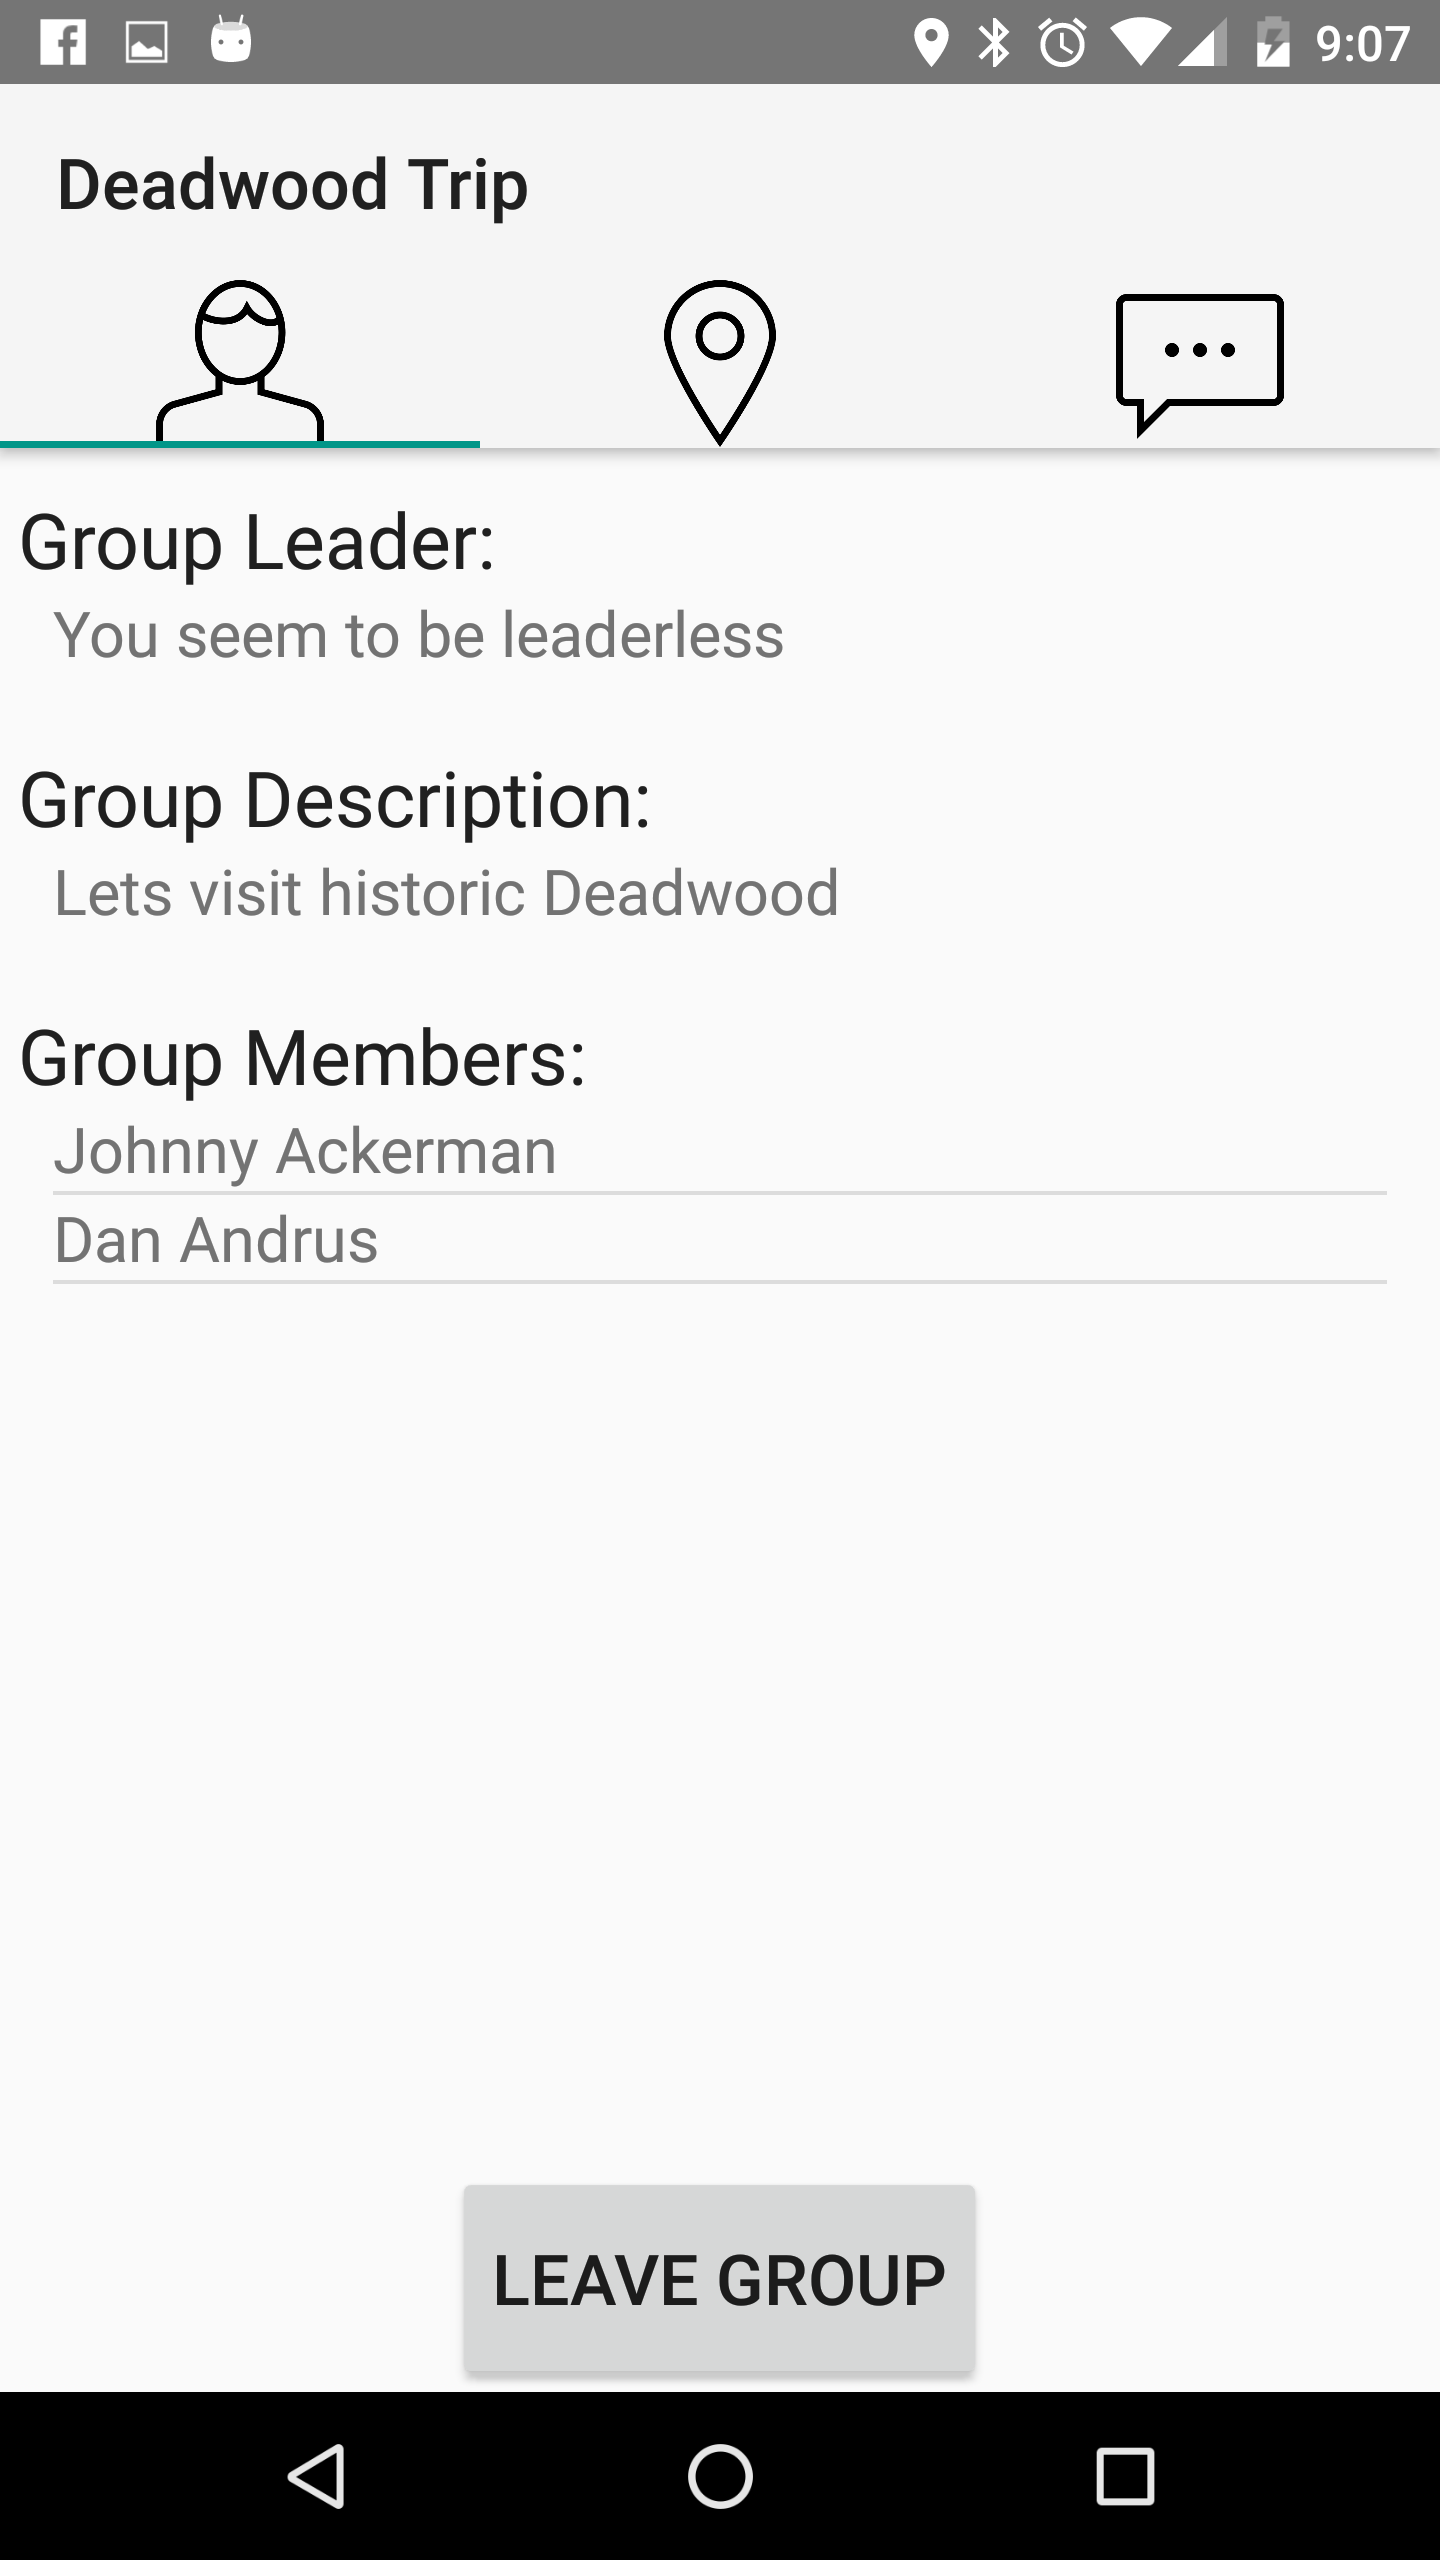
\includegraphics[scale=.1]{Additional/Prototypes/Sprint5/groupInfo.PNG}}
	\fbox{\includegraphics[scale=.1]{Additional/Prototypes/Sprint5/leaving.PNG}}
	\fbox{\includegraphics[scale=.1]{Additional/Prototypes/Sprint5/login.PNG}}
	\fbox{\includegraphics[scale=.1]{Additional/Prototypes/Sprint5/map.PNG}}
	\fbox{\includegraphics[scale=.1]{Additional/Prototypes/Sprint5/messaging.PNG}}
	\end{center}
	\caption{Sprint 5 Prototypes. \label{CommFlow}}
	\end{figure}

\subsection{Deliverable}
\begin{itemize}
	\item Android
	\begin{itemize}
		\item Group Messaging
		\begin{itemize}
			\item Discovered and removed a bug
		\end{itemize}
	\item Location
	\begin{itemize}
		\item Moved remote functionality to model manager
		\item Updated location model to reflect changes
		\item Caching objects
	\end{itemize}
		\item App Appearance
		\begin{itemize}
			\item Reformatted the entire theme of the app (all pages are based of the same theme now - no more custom themes per page)
			\item Added a tool bar to the group join page/ removed settings button (now in tool bar)
			\item Group Information Page
			\begin{itemize}
				\item Added a group leader display
				\item Added padding to appearance of display and modified text sizes
				\item Displays all group members
				\item Displays Dialog box if user attempts to leave the group
			\end{itemize}
		\end{itemize}
	\end{itemize}
	\item Server (cloud code)
	\begin{itemize}
		\item Join function
		\item Leave function
	\end{itemize}
	\item Misc/Transitional
	\begin{itemize}
		\item Business Plan revised and submitted to The Governor's Giant Vision Competition
		\item Finalist for The Governor's Giant Vision Competition
		\item Some of the overall Senior Design Doc has been touched up
	\end{itemize}
\end{itemize}
\subsection{Backlog}
\begin{itemize}
	\item Senior Design Doc
	\begin{itemize}
		\item Do a general revision of the doc
	\end{itemize}
	\begin{itemize}
		\item Business Plan
		\begin{itemize}
			\item Finish business plan for 2016 Governor's Giant Vision Competition
		\end{itemize}
	\end{itemize}
	\item Android
	\begin{itemize}
		\item Model Caching/ Uniformity
		\item Clean up appearance
		\item Clean up the appearance of the app
		\item Display Group Members on group info page
		\item Safe group operations(leaving/joining group)
		\item Loading animations on homing and syncing
		\item Integration Testing
		\item Start Alpha Testing
	\end{itemize}
	\item Cloud code
	\begin{itemize}
		\item Safe group operations(leaving/joining group)
		\item test join and leave functionality
	\end{itemize}
\end{itemize}
\subsection{Success/Fail}
\begin{itemize}
	\item Failures
	\begin{itemize}
		\item Android
		\begin{itemize}
			\item Messaging still needs an appearance update for usability
		\end{itemize}
		\begin{itemize}
			\item Cloud Code
			\begin{itemize}	
				\item Needs more testing on group functions
				\item Completing join and leave functions
			\end{itemize}
		\end{itemize}
	\end{itemize}
	\item Successes
	\begin{itemize}
		\item Added safe group operations though cloud code
		\item Reformatted the theme of the app
		\item Added tool bar to tab section of groups
		\item Finalist for The Governor's Giant Vision Competition
		\item Fixed a few bugs in the location code
	\end{itemize}
\end{itemize}


\section{Sprint 6 Prototype}

	\begin{figure}[tbh]
	\begin{center}
	\fbox{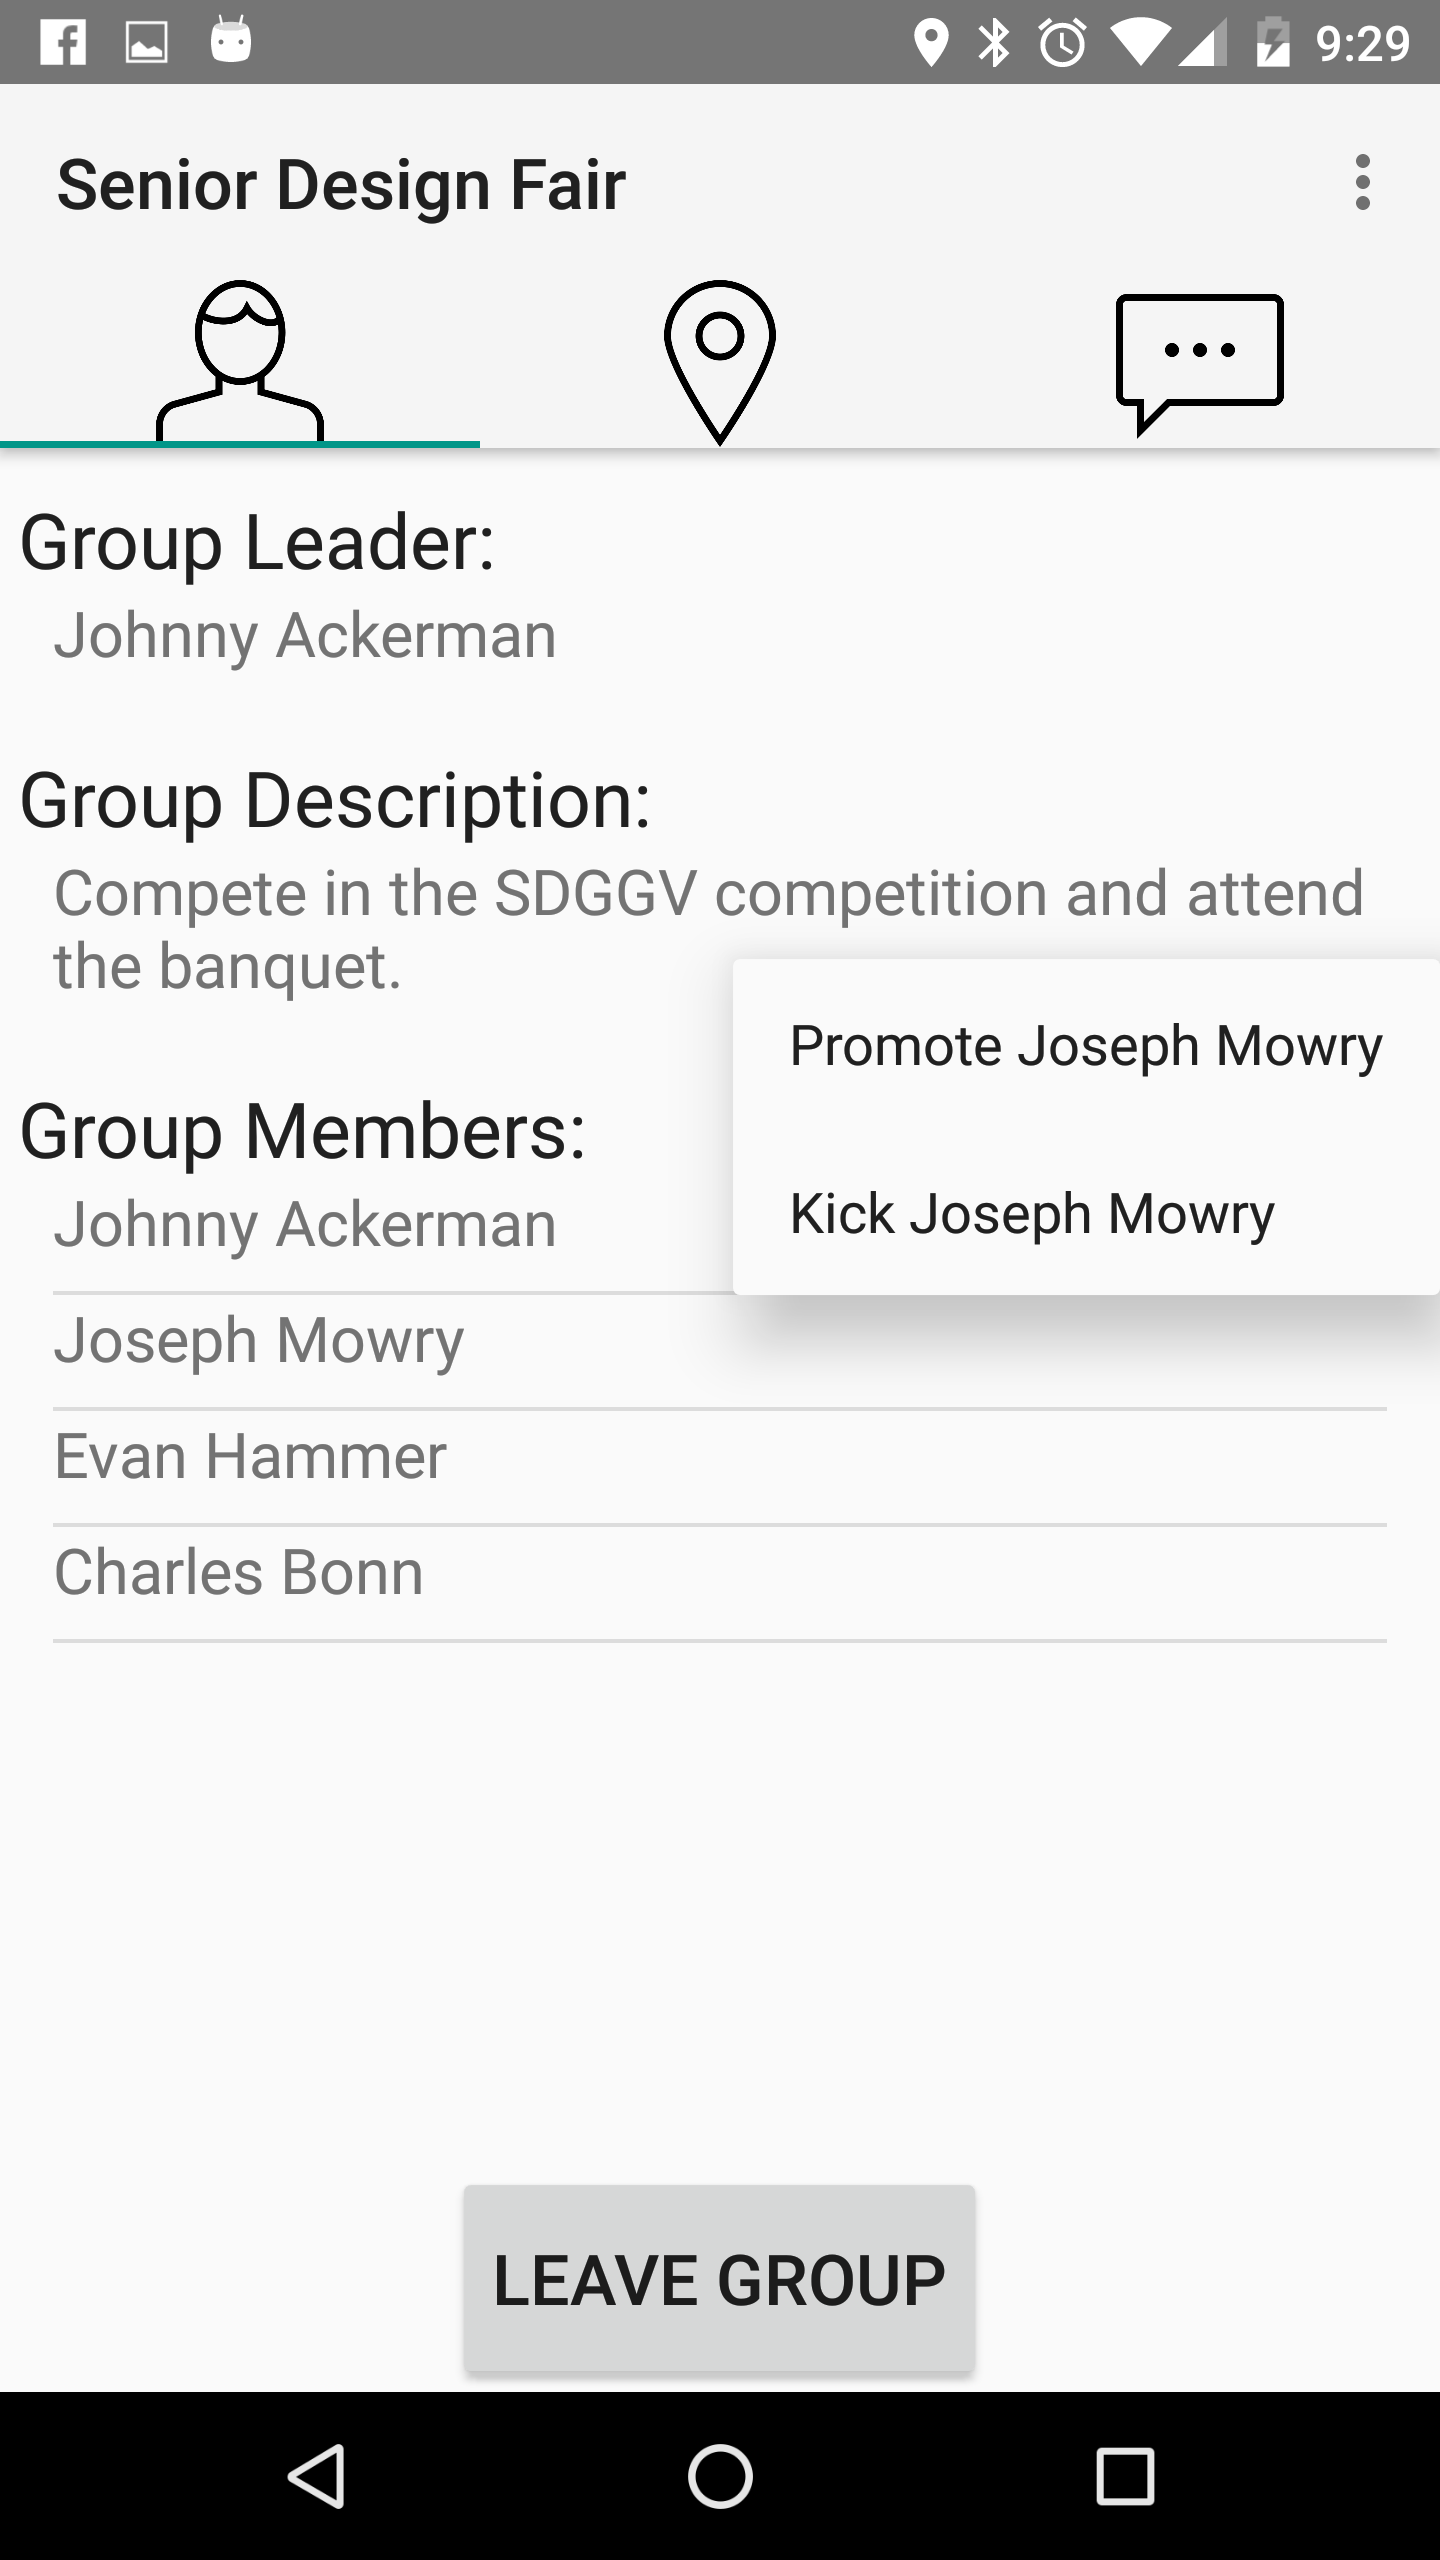
\includegraphics[scale=.1]{Additional/Prototypes/Sprint6/commands.PNG}}
	\fbox{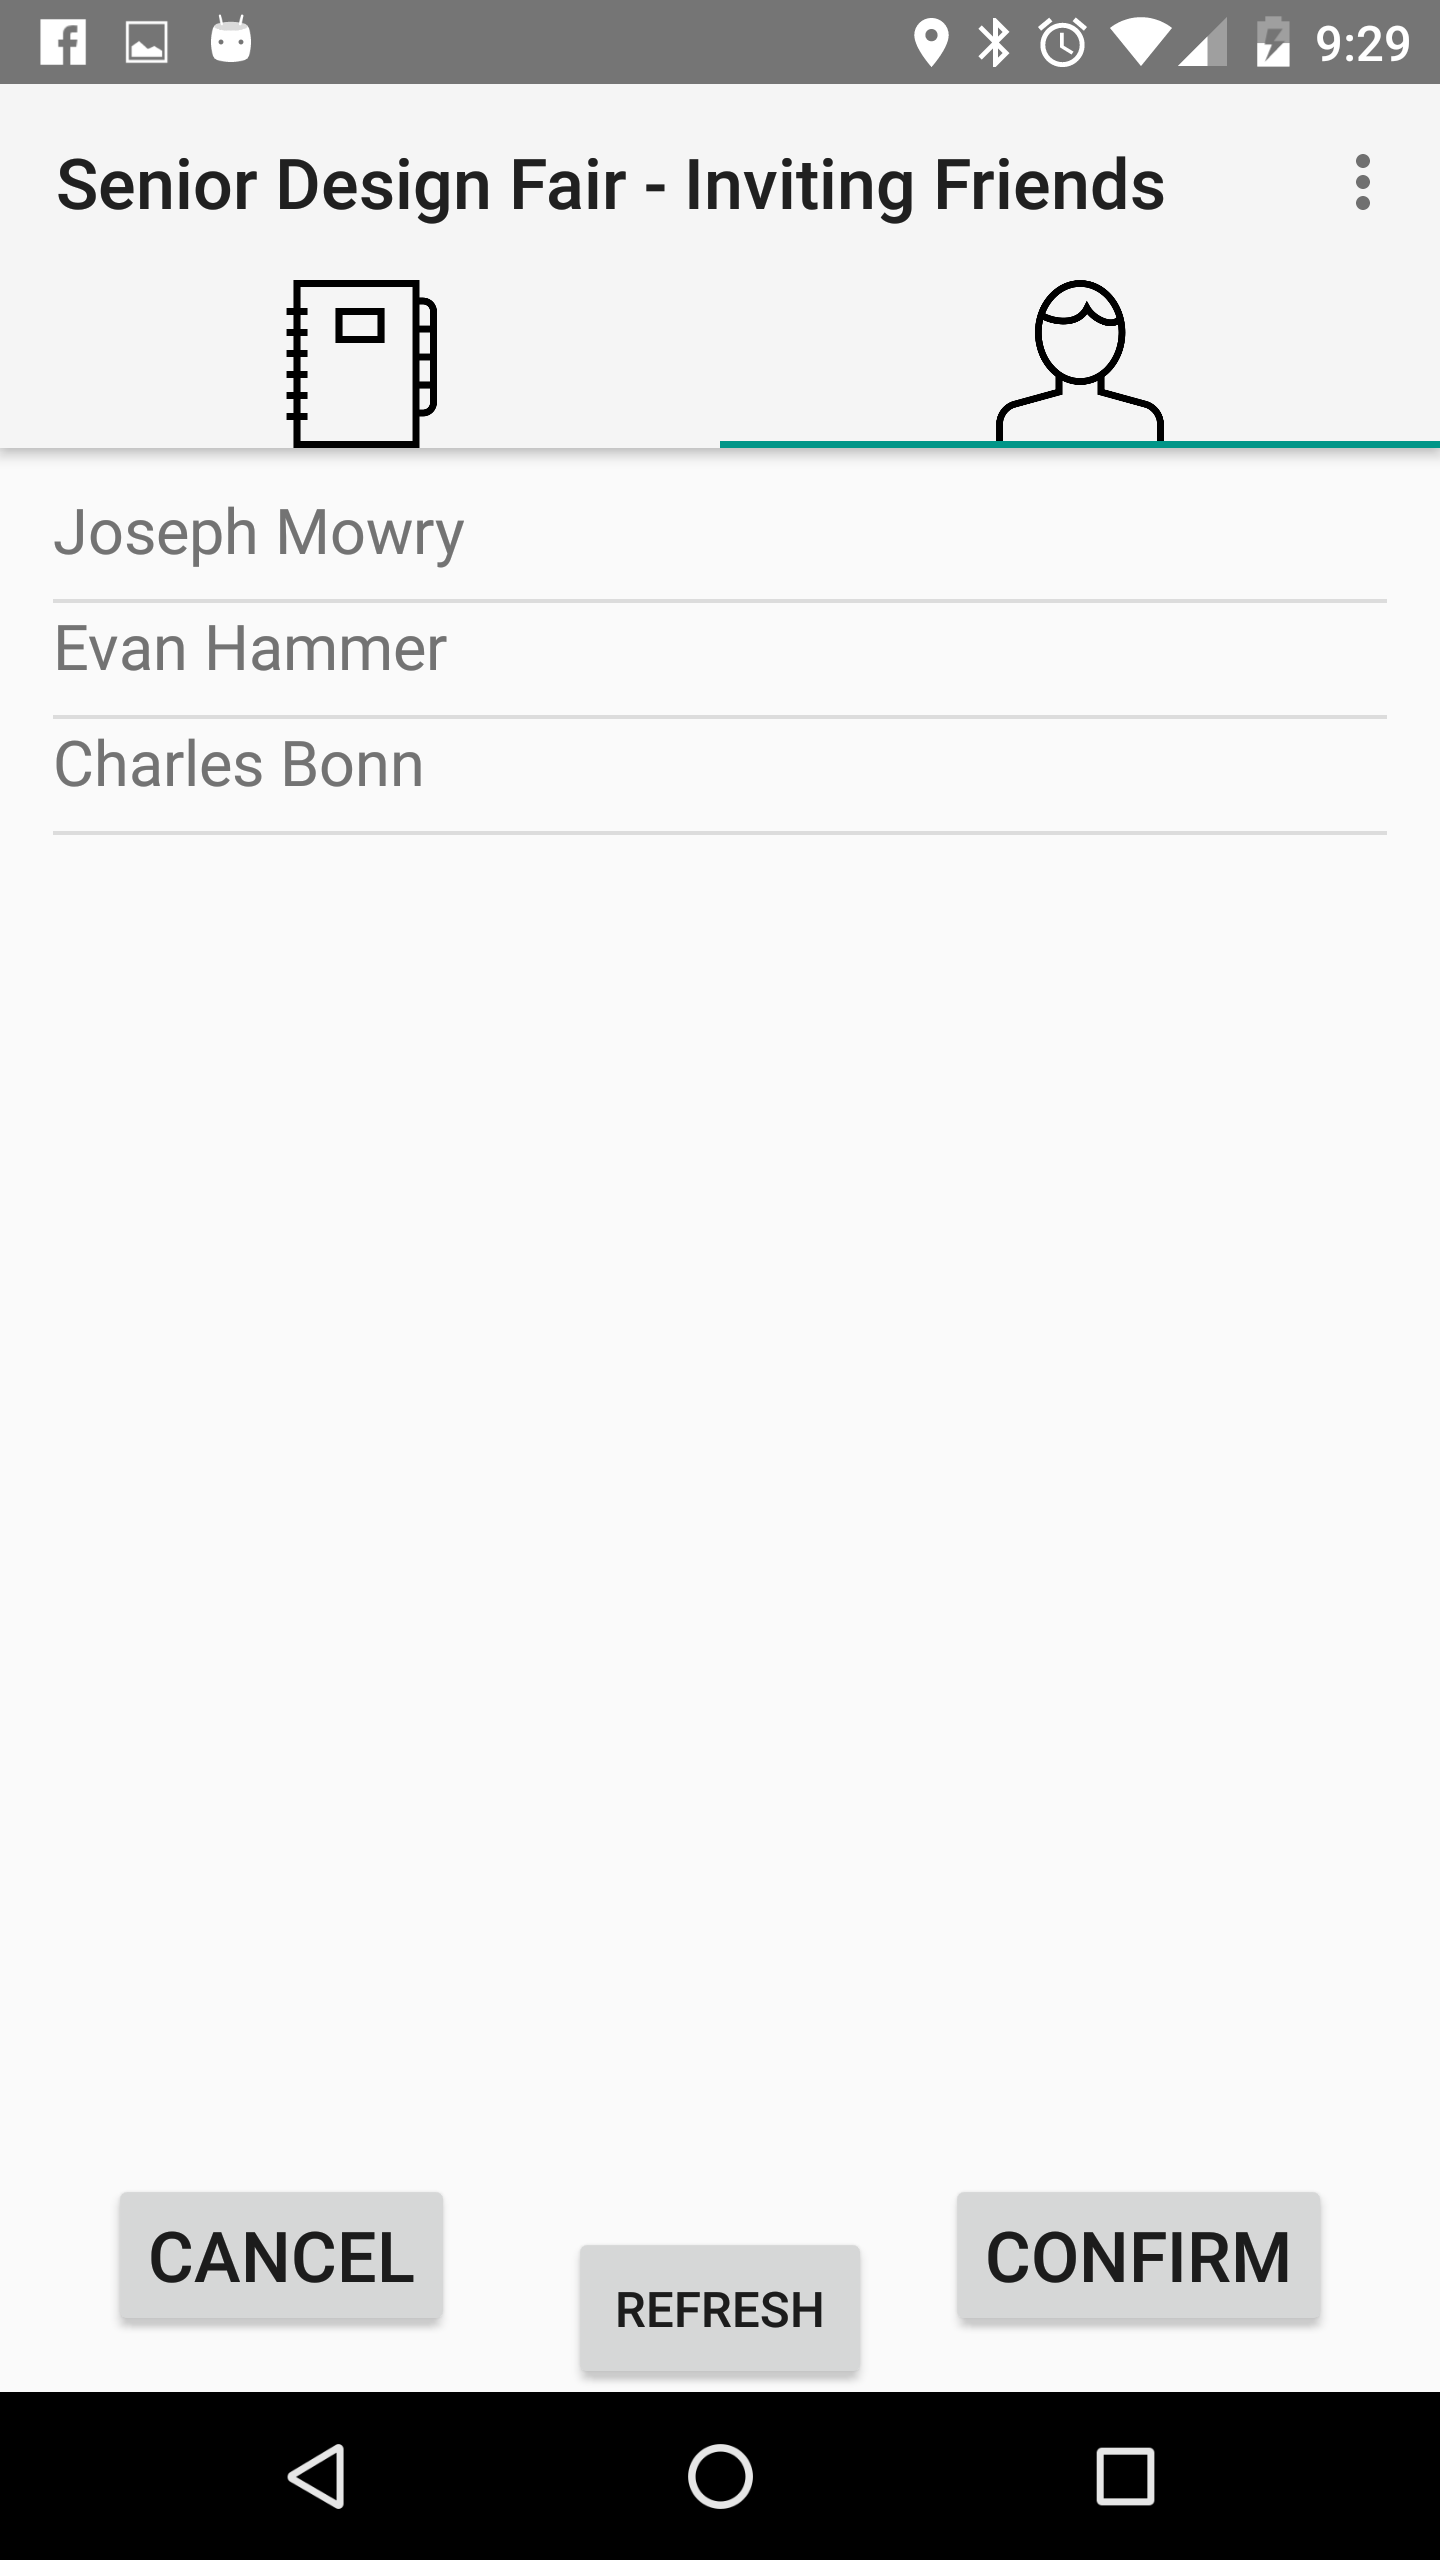
\includegraphics[scale=.1]{Additional/Prototypes/Sprint6/confirm.PNG}}
	\fbox{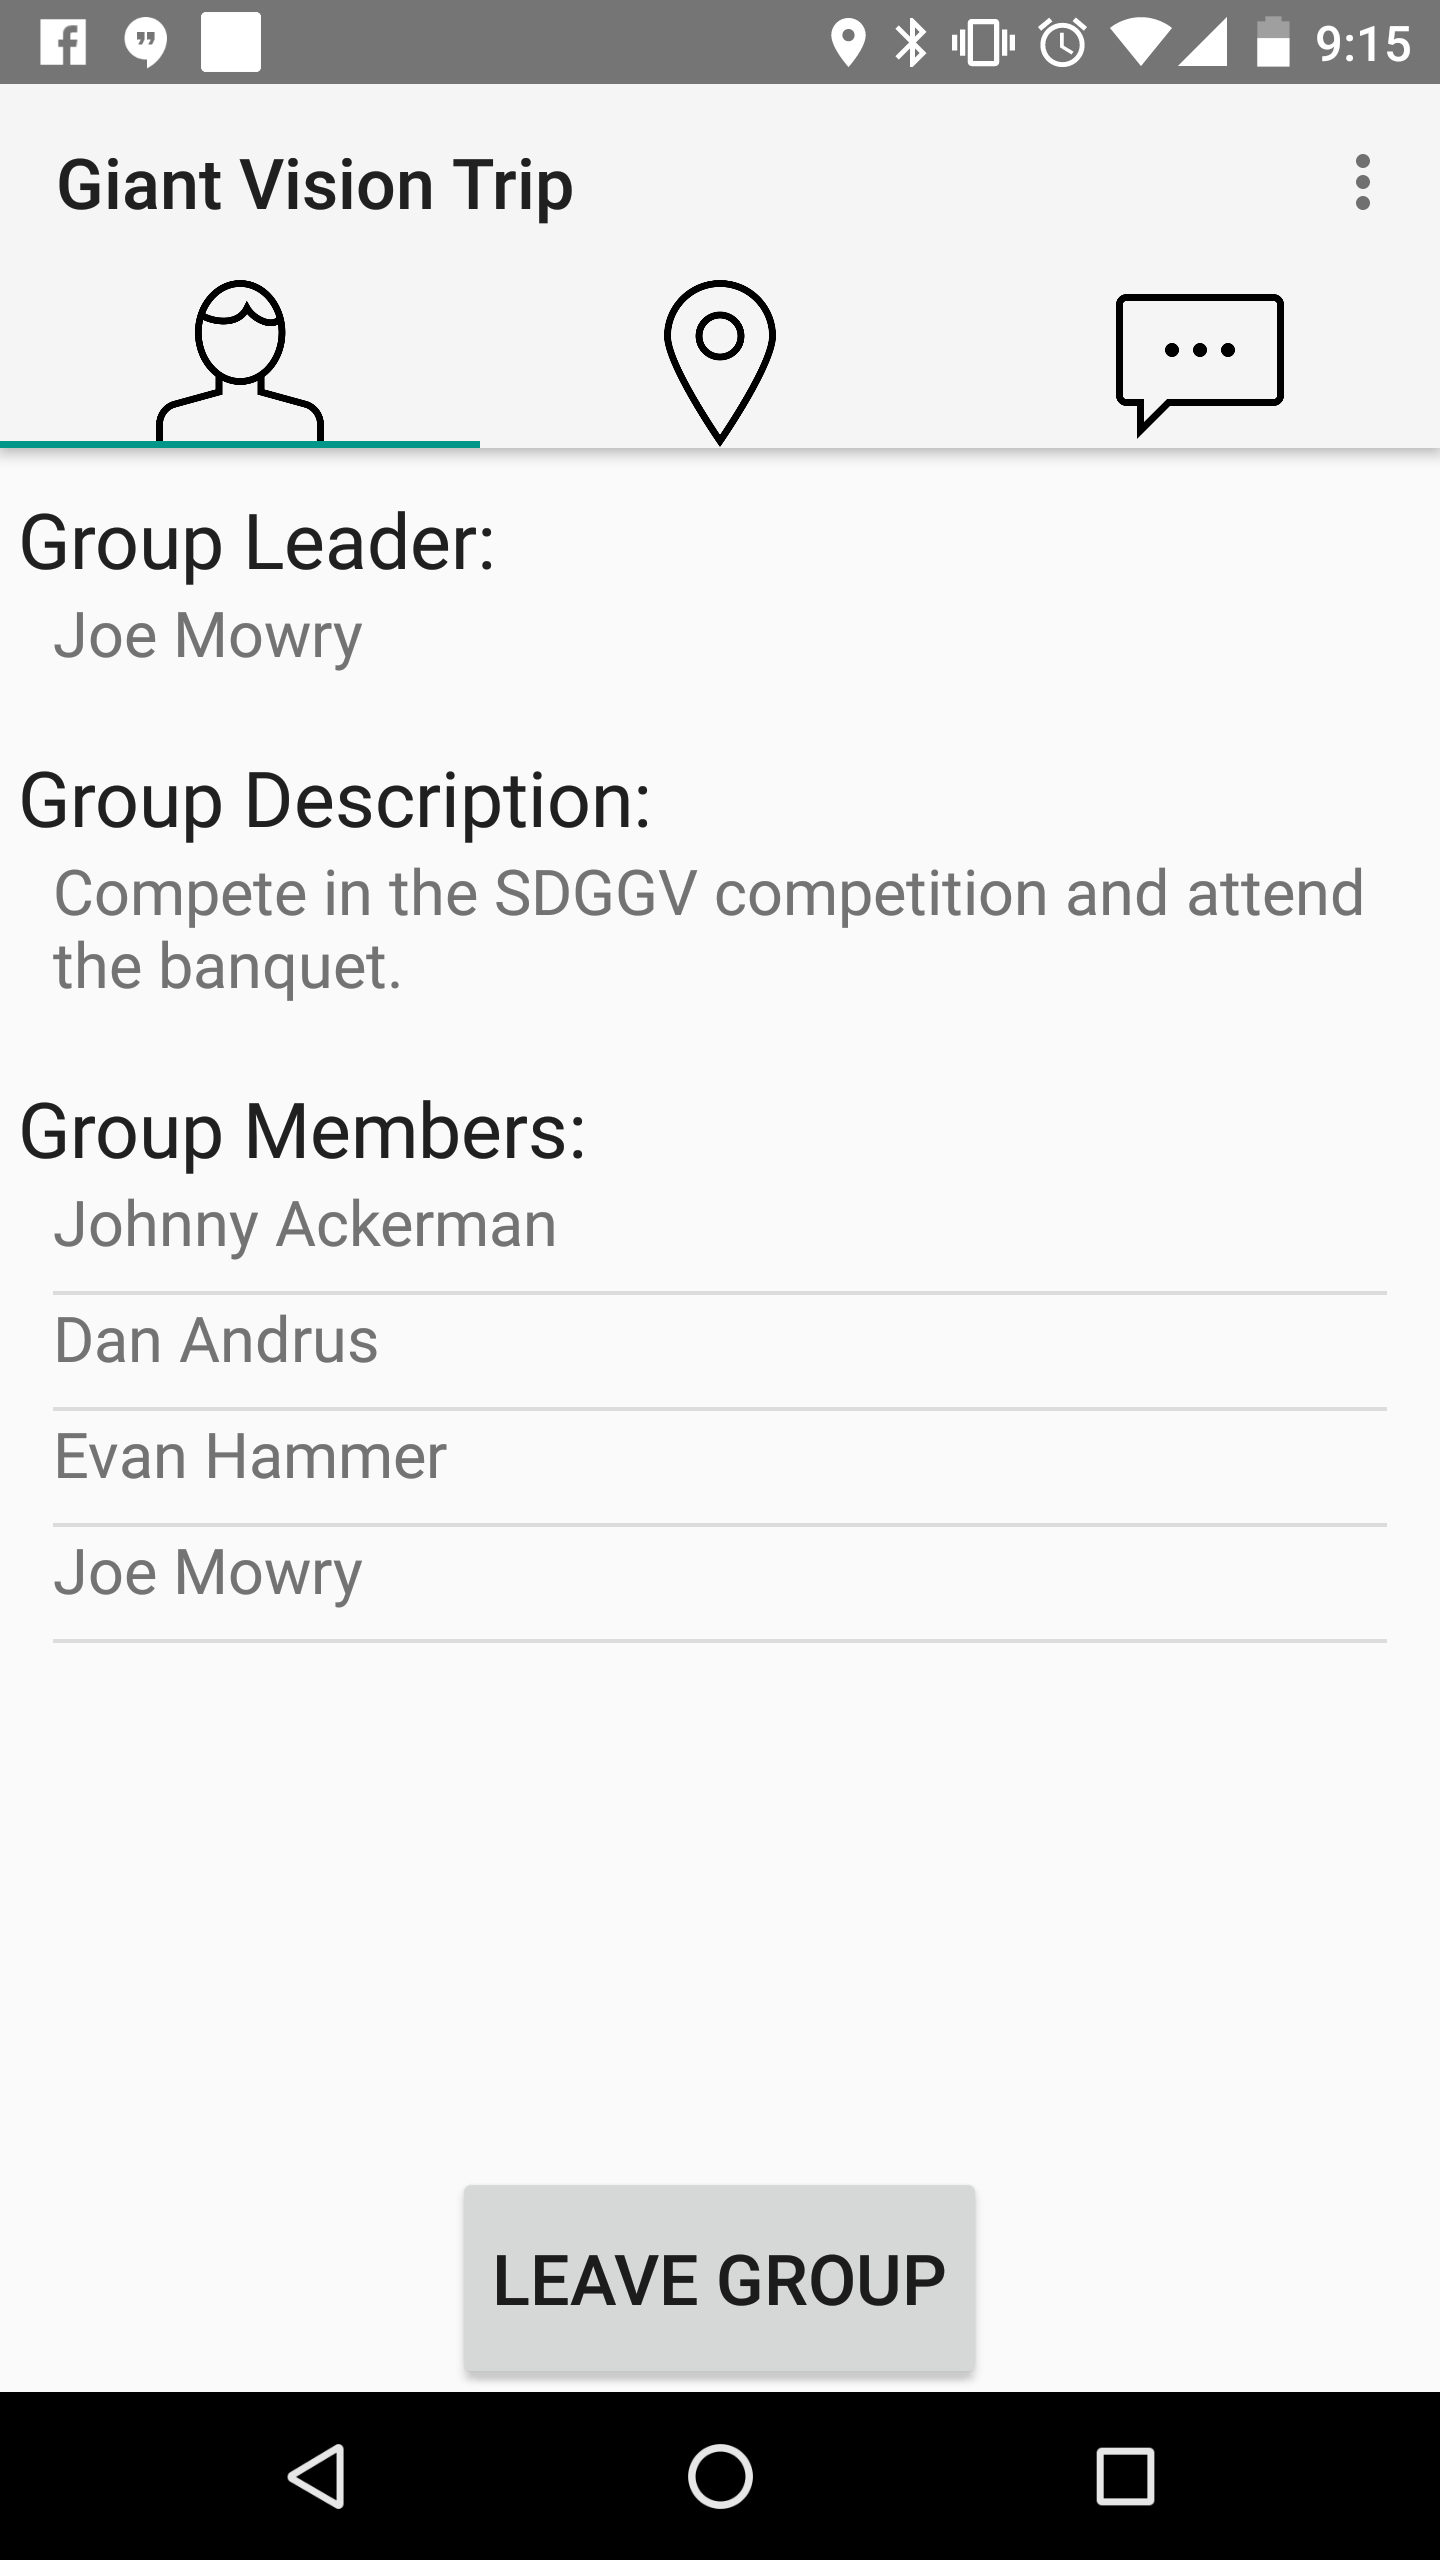
\includegraphics[scale=.1]{Additional/Prototypes/Sprint6/groupActivity.PNG}}
	\fbox{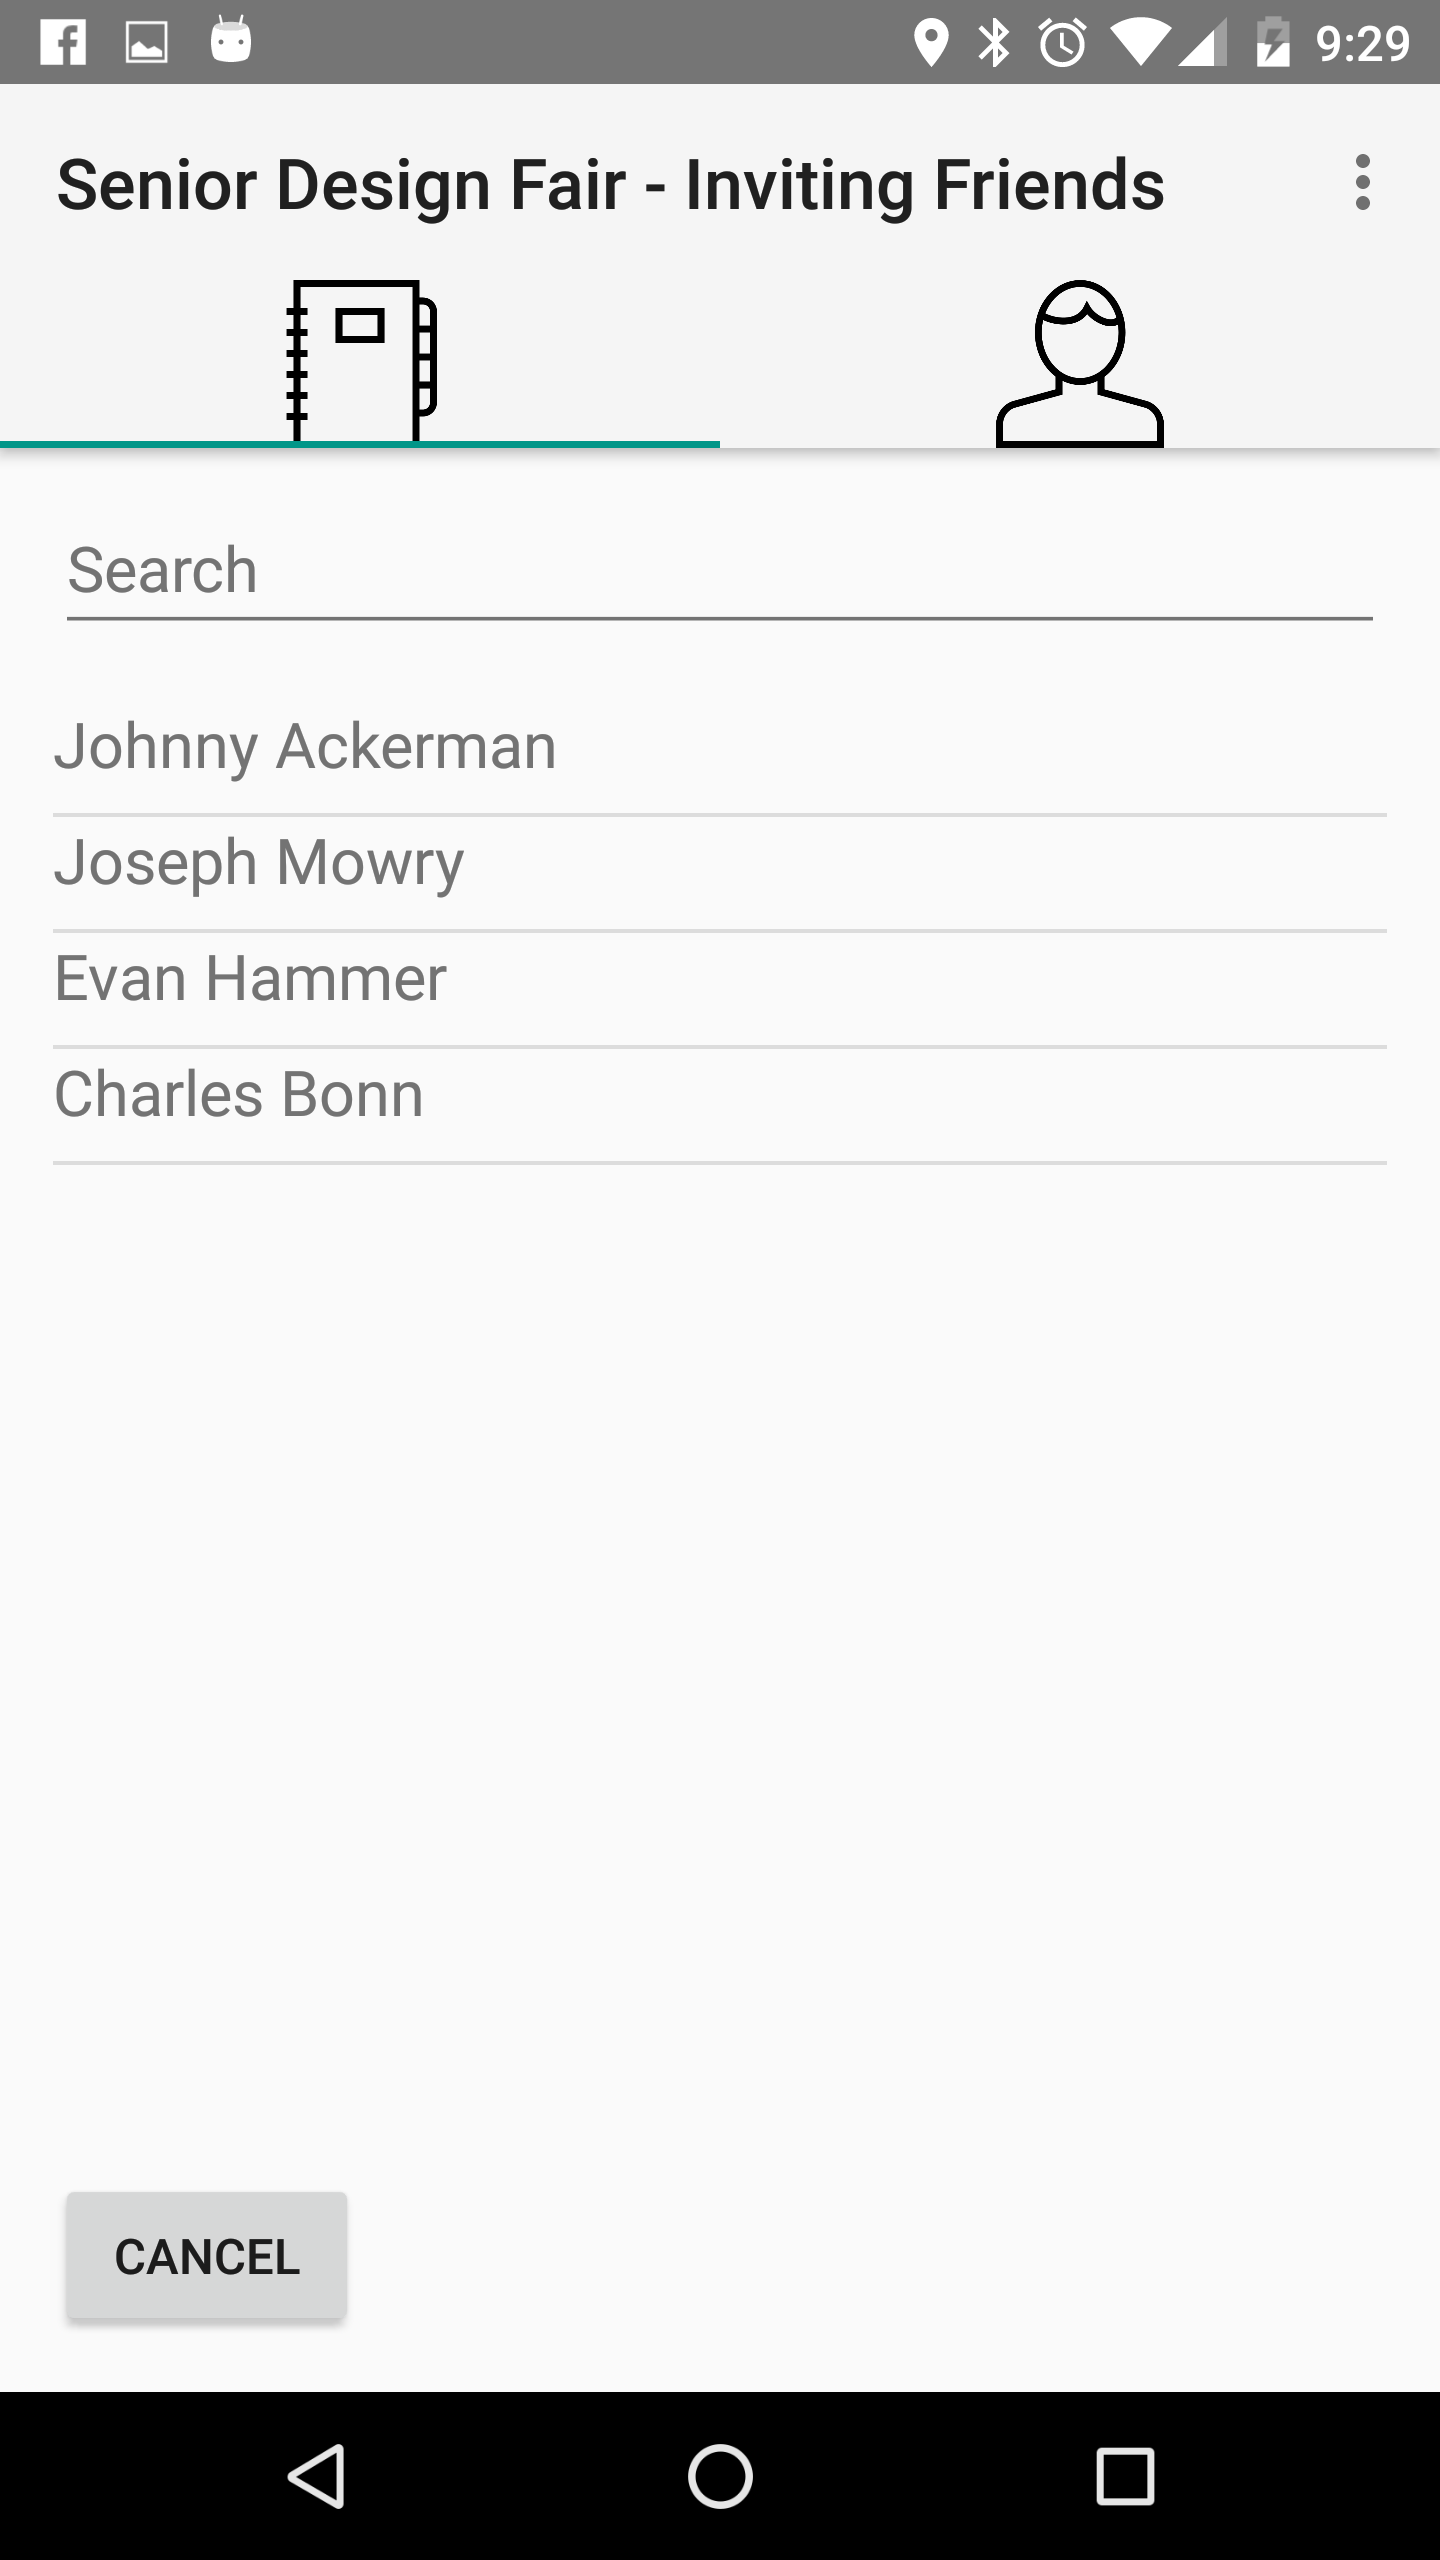
\includegraphics[scale=.1]{Additional/Prototypes/Sprint6/invite.PNG}}
	\fbox{\includegraphics[scale=.1]{Additional/Prototypes/Sprint6/leaving.PNG}}
	\fbox{\includegraphics[scale=.1]{Additional/Prototypes/Sprint6/logIn.PNG}}
	\fbox{\includegraphics[scale=.1]{Additional/Prototypes/Sprint6/map.PNG}}
	\fbox{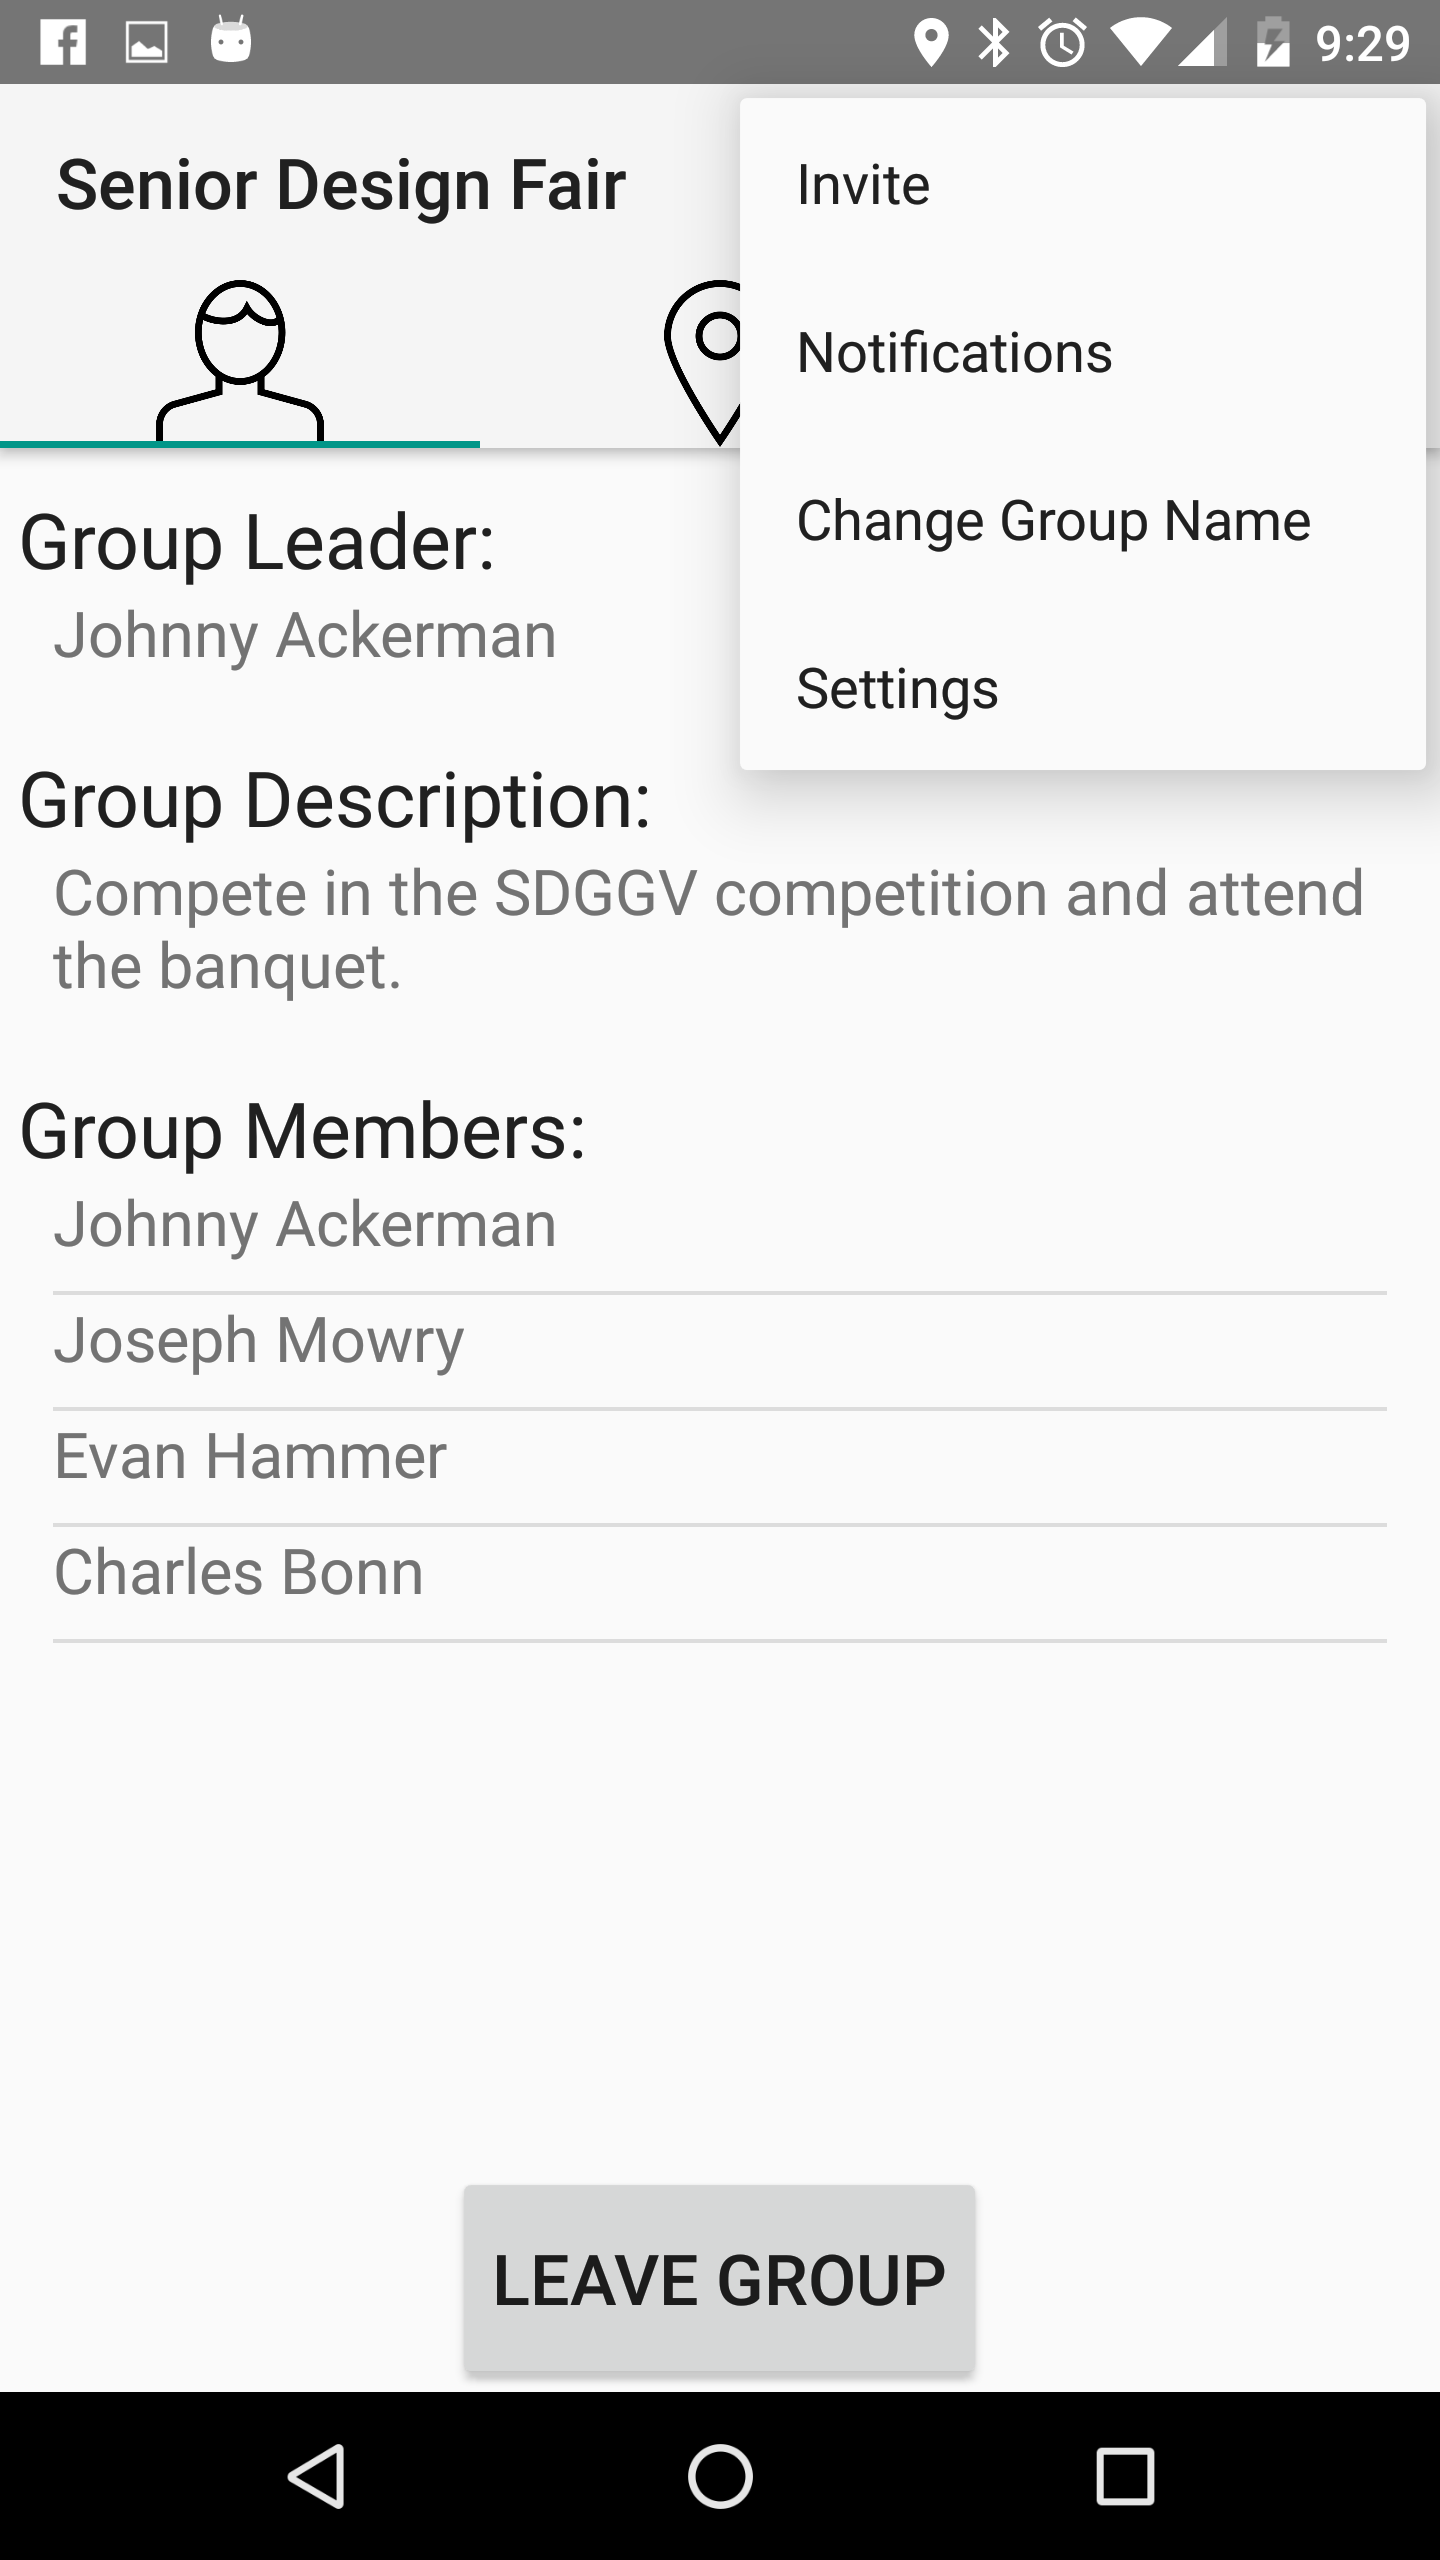
\includegraphics[scale=.1]{Additional/Prototypes/Sprint6/menu.PNG}}
	\fbox{\includegraphics[scale=.1]{Additional/Prototypes/Sprint6/messaging.PNG}}
	\fbox{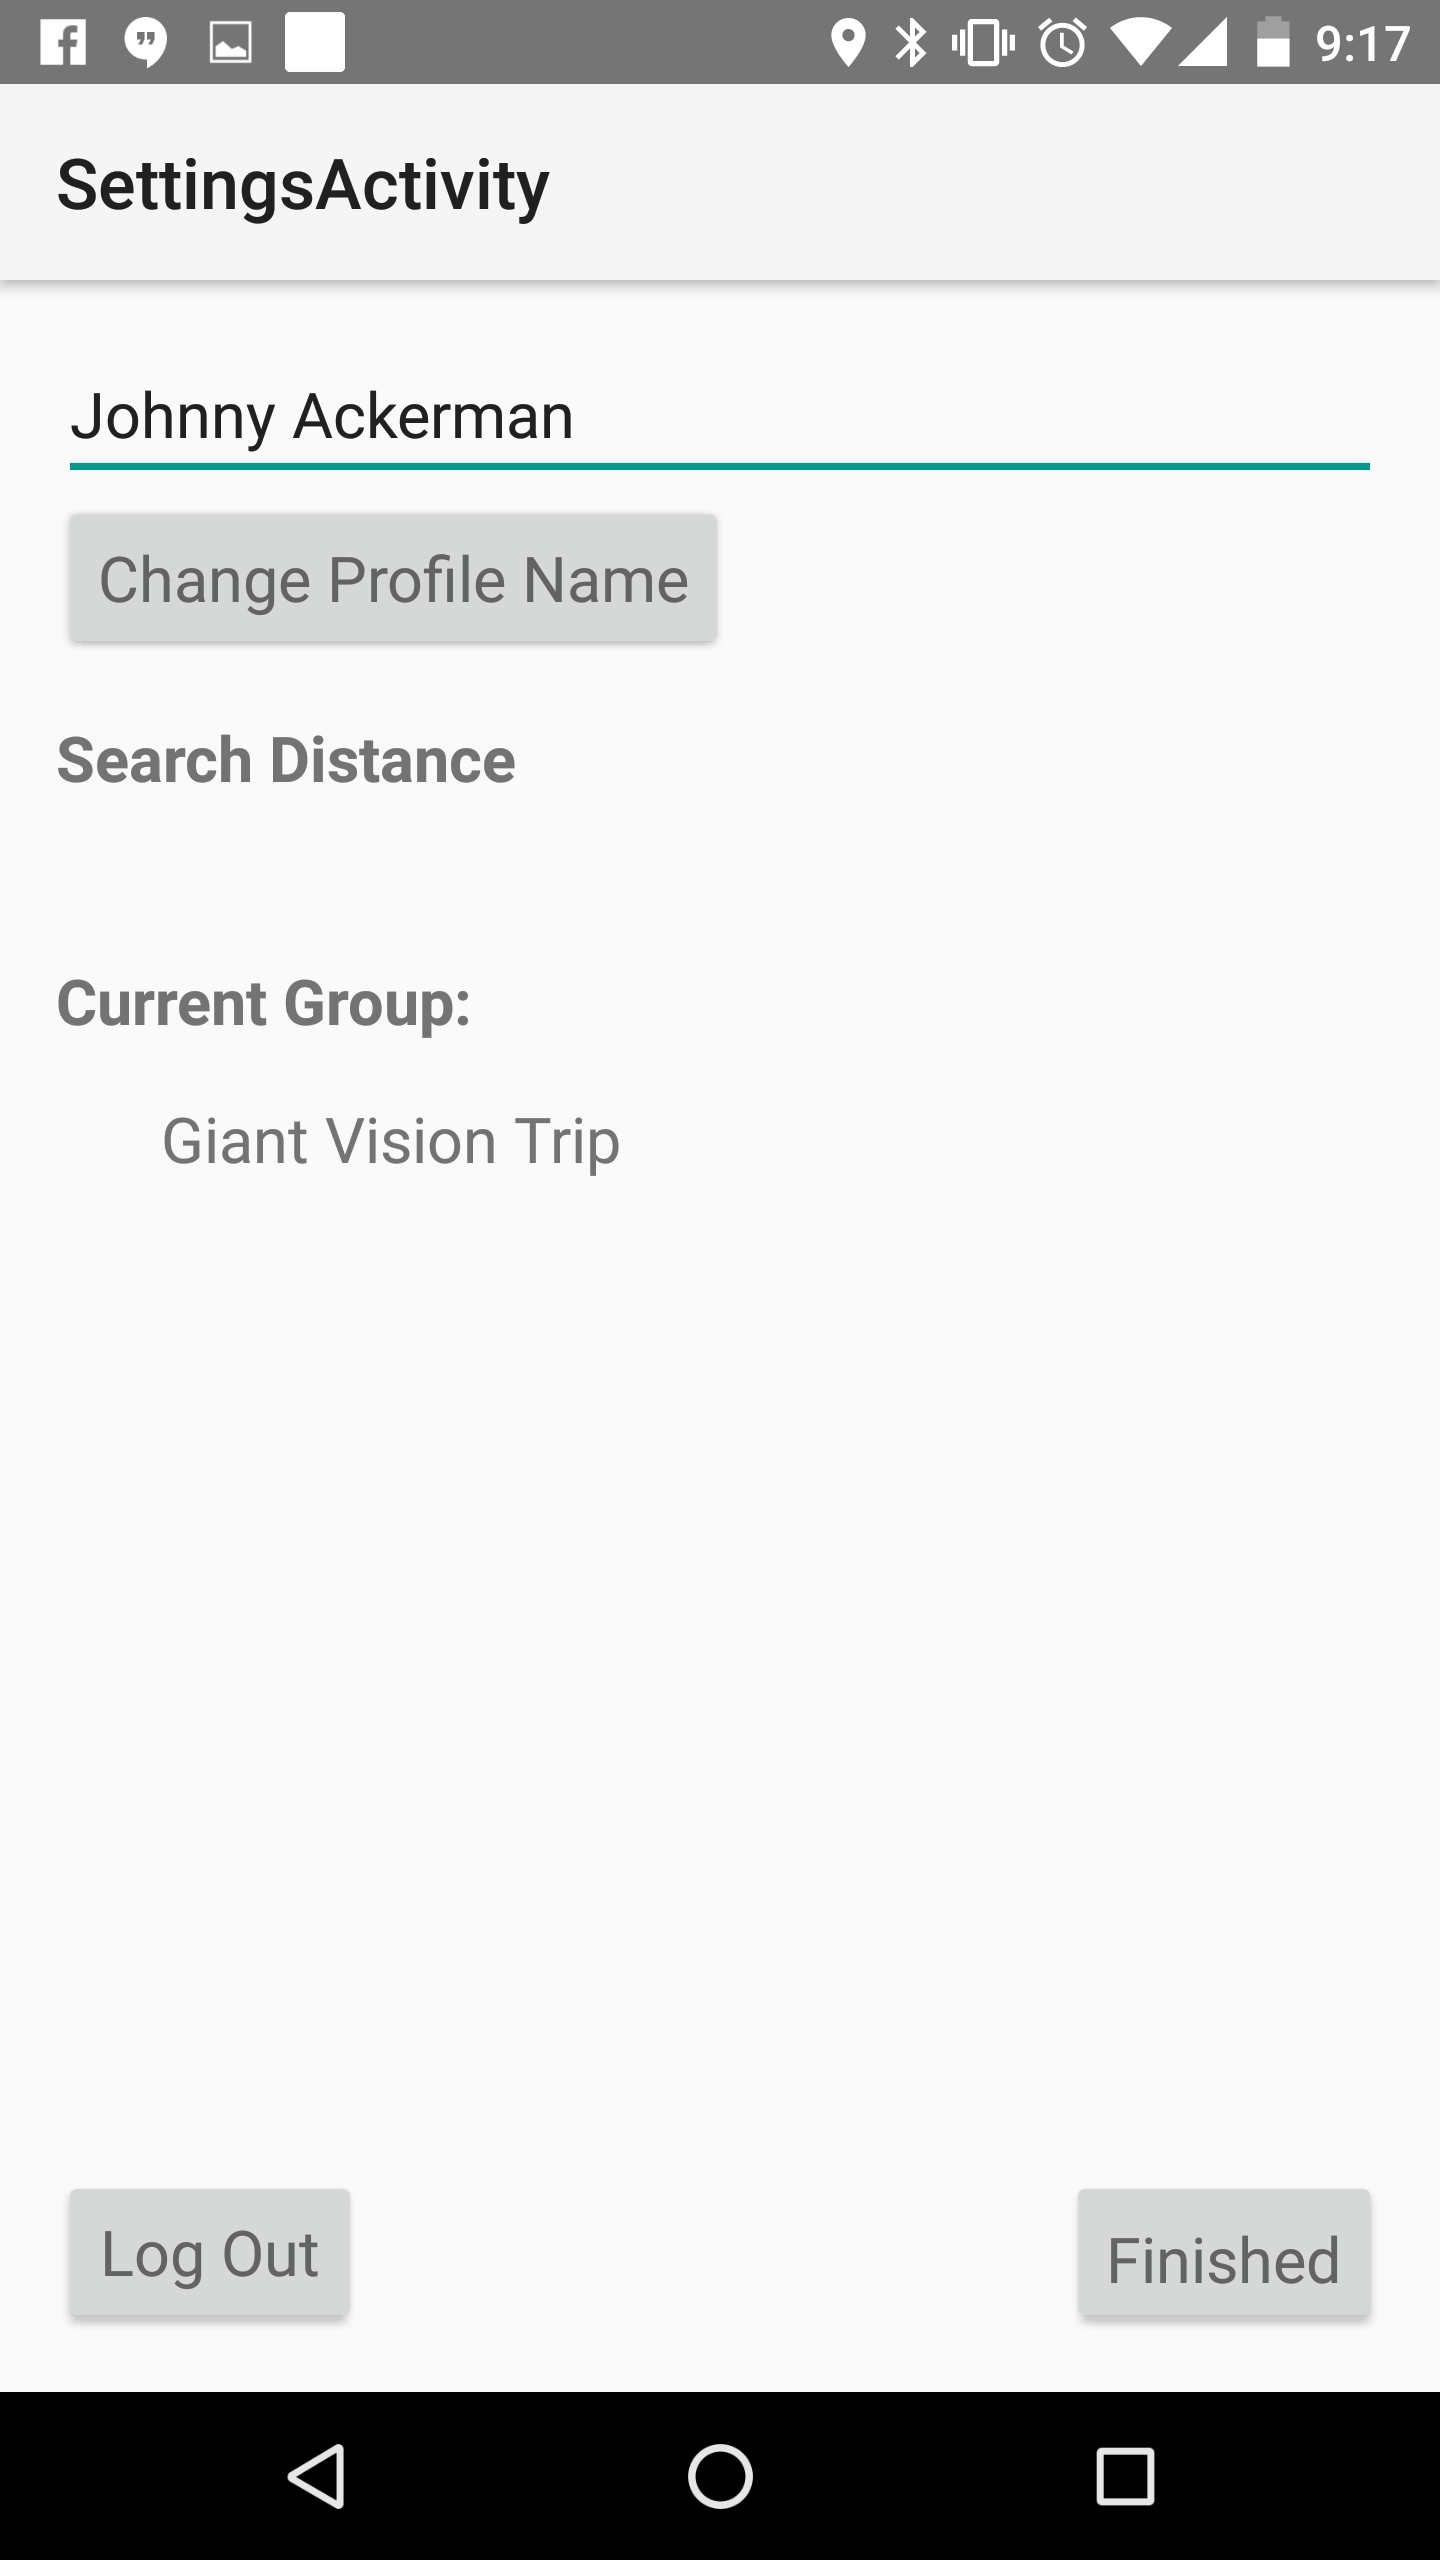
\includegraphics[scale=.1]{Additional/Prototypes/Sprint6/settings.PNG}}
	\end{center}
	\caption{Sprint 6 Prototypes. \label{CommFlow}}
	\end{figure}

\subsection{Deliverable}
\begin{itemize}
	\item Android
	\begin{itemize}
		\item Group Messaging
		\begin{itemize}
			\item Messages now include the names of the sender
			\item Leader can now kick or promote members
			\item Messages now load per group from parse
		\end{itemize}
		\item broke ground for notification system
		\begin{itemize}
			\item created tab system for invites and accepts
			\item created fragments for invite and confirm
			\item created model for notification system
			\item items can be transferred from the invite fragment to the confirm fragment
		\end{itemize}
		\item Group Management Tools
		\begin{itemize}
			\item Leader can now kick a member
			\item Leader can now promote a member
			\item fixed leader bug, now leader loads properly
		\end{itemize}
	\end{itemize}
\end{itemize}
\subsection{Backlog}
\begin{description}
	\item[Week 1] \hfill
	\begin{itemize}
		\item Android
		\begin{itemize}
			\item Messaging
			\begin{itemize}
				\item Messages now include the names of the sender
				\item Leader can now kick or promote members
				\item Messages now load per group from parse
			\end{itemize}
			\item Group Management Tools
			\begin{itemize}
				\item Leader can now kick a member
				\item Leader can now promote a member
			\end{itemize}
			\item Facebook and Twitter log-in
		\end{itemize}
	\end{itemize}
	
  \item[Week 2] \hfill
		\begin{itemize}
		\item Android
		\begin{itemize}
			\item fixed leader bug, now leader loads properly
			\item broke ground for notification system
			\begin{itemize}
				\item created tab system for invites and accepts
				\item created fragments for invite and confirm
				\item created model for notification system
				\item items can be transferred from the invite fragment to the confirm fragment
			\end{itemize}
			\item Option Menu's added 
			\begin{itemize}
				\item group join now has an option menu
				\item settings activity moved to option menu
				\item Group name can be changed in option menu
				\item option menu is different if you are a group leader
				\item option menu leads to invite system
				\item option menu leads to blank notification page
			\end{itemize}
			\item Reformatted settings activity
			\begin{itemize}
				\item now displays and can change display name
				\item displays a current group if in one
				\item added a finish button for clarity
			\end{itemize}
		\end{itemize}
		\item Cloud code
		\begin{itemize}
			\item Safe group operations(leaving/joining group)
		\end{itemize}
	\end{itemize}
  
  \item[Week 3] \hfill
		\begin{itemize}
		\item Giant Vision Competition
		\begin{itemize}
			\item demonstrated the project and started collecting users for beta
		\end{itemize}
		\item Android
		\begin{itemize}
			\item Notification and invite system incomplete
		\end{itemize}
	\end{itemize}
\end{description}

\subsection{Success/Fail}
\begin{itemize}
	\item Android
	\begin{itemize}
		\item Facebook and Twitter log-in incomplete
		\item Notification and invite system incomplete
	\end{itemize}
	\item Misc
	\begin{itemize}
		\item Did not place at the Giant Vision Competition
	\end{itemize}
\end{itemize}

